% Use only LaTeX2e, calling the article.cls class and 12-point type.

\documentclass[12pt]{article}

% Users of the {thebibliography} environment or BibTeX should use the
% scicite.sty package, downloadable from *Science* at
% www.sciencemag.org/about/authors/prep/TeX_help/ .
% This package should properly format in-text
% reference calls and reference-list numbers.

\usepackage{scicite}
\usepackage{float}
\usepackage{pgfplots}
\usepackage{pgfplotstable}
\usepackage{graphicx}
\usepackage{wrapfig}
\usepackage{xcolor}

\usepackage{placeins} % For floatbarrier
\usepackage{hyperref} % For urls
\usepackage{float}    % To place images on spot
\usepackage{gensymb}  % For using the degree symbol

% Use times if you have the font installed; otherwise, comment out the
% following line.

\usepackage{times}

% The preamble here sets up a lot of new/revised commands and
% environments.  It's annoying, but please do *not* try to strip these
% out into a separate .sty file (which could lead to the loss of some
% information when we convert the file to other formats).  Instead, keep
% them in the preamble of your main LaTeX source file.


% The following parameters seem to provide a reasonable page setup.

\topmargin 0.0cm
\oddsidemargin 0.2cm
\textwidth 16cm
\textheight 21cm
\footskip 1.0cm


\newenvironment{changemargin}[2]{%
\begin{list}{}{%
\setlength{\topsep}{0pt}%
\setlength{\leftmargin}{#1}%
\setlength{\rightmargin}{#2}%
\setlength{\listparindent}{\parindent}%
\setlength{\itemindent}{\parindent}%
\setlength{\parsep}{\parskip}%
}%
\item[]}{\end{list}}

%The next command sets up an environment for the abstract to your paper.

\newenvironment{sciabstract}{%
\begin{quote} \bf}
{\end{quote}}


% If your reference list includes text notes as well as references,
% include the following line; otherwise, comment it out.

%\renewcommand\refname{References and Notes}


% Include your paper's title here

\title{Micromouse: Designing an Educational Racing-Robot from Scratch \\Report}



% Place the author information here.  Please hand-code the contact
% information and notecalls; do *not* use \footnote commands.  Let the
% author contact information appear immediately below the author names
% as shown.  We would also prefer that you don't change the type-size
% settings shown here.

% I think we should organize our names alphabetically
\author
{Adam Pasvatis$^{1}$, Frank ...$^{2}$, Meryem Guemimi$^{3}$, Natalia Poliakova$^{4}$, René Lalla$^{5}$, Sihong Chen$^{6}$\\
\\
\normalsize{$^{1}$Department of Informatics, Technical University of Munich, Matriculation Number: 03707465}\\
\normalsize{$^{2}$Department of Informatics, Technical University of Munich, Matriculation Number: XXXXXXXX}\\
\normalsize{$^{3}$Department of Informatics, Technical University of Munich, Matriculation Number: 03713693}\\
\normalsize{$^{4}$Department of Informatics, Technical University of Munich, Matriculation Number: 03682089}\\
\normalsize{$^{5}$Department of Informatics, Technical University of Munich, Matriculation Number: 03694669}\\
\normalsize{$^{6}$Department of Informatics, Technical University of Munich, Matriculation Number: 03691664}\\
\\
}

% Include the date command, but leave its argument blank.

\date{}



%%%%%%%%%%%%%%%%% END OF PREAMBLE %%%%%%%%%%%%%%%%



\begin{document}

% Double-space the manuscript.

\baselineskip24pt

% Make the title.

\maketitle

\newpage

% Place your abstract within the special {sciabstract} environment.
\begin{sciabstract}
  \section*{Abstract}
    This project was about designing and building a robotic "mouse" which is able to find the center of a maze autonomously. The idea was inspired by a competition called "Micromouse" which is held in various countries.

    In order to gain the required knowledge and grasp the complexity of the challenge, it was necessary to learn detailed information about all used electrical components and the tools to actually implement them - which is described in the first chapters.

    The main purpose of this project was to understand the several concepts of how electrical components interact and interfere with each other and how to write software for a microcontroller which lets it control its attached motors to be able to drive autonomously.

    Furthermore, it was crucial to know how you have to design a PCB which looks clean, has no unnecessary tracing-loops to avoid electo-magnetic induction and doesn't exceed its specified dimensions.\\

    \noindent
    The result is, unfortunately, a half-finished robot. The software is written, the casing is done and the electrical parts are ordered. But the parts still need to be soldered onto the PCB, the sensors need to be adjusted and the software has to be tested on the final assembled robot.\\

\end{sciabstract}

\newpage

\Large \textbf{Contribution to the project}\\

\normalsize Short description of how each Micromouse project member contributed to the final result.

\begin{itemize}
    \item Adam\\
        Code for the old microcontroller, Schematic, PCB Design, Components Order, The entire Hardware part in the report except for Casing section
    \item Frank\\
    \item Meryem\\
        initial software configuration together with Frank (pin mapping, GPIO, configuration bits), peripheral configuration: timer, ADC, DMA, motor driving functions together with Frank, PID controller: implementation of a cascade controller.
    \item Natalia\\
        In the first ("acquiring basic knowledge") half of the semester, due to the previous experience in embedded programming, I was mainly focused on helping other project members to grasp various concepts that were new to them, answering questions regarding the material and implementing the prototypes from weekly exercises on the breadboard.
        After the group reorganization (which followed shortly after the actual work on building the micromouse started) I joined the hardware team and with other team members worked on the first versions of schematics design, performed the initial PCB tracing, contributed to maintaining the component ordering and description tables.
        Moreover, I tried to help other teams whenever possible as well as to maintain the connection between teams and inform everyone of the current progress.
    \item René\\
         Design of the schematic and PCB, finding electrical components via SamacSys Library for Autodesk Eagle, tracing of the PCB
    \item Sihong\\
        Casing design, 3D printing, components order. In this report, chapter of Fusion 360 workshop, as well as anything related to the casing.
\end{itemize}


\newpage

\tableofcontents



% In setting up this template for *Science* papers, we've used both
% the \section* command and the \paragraph* command for topical
% divisions.  Which you use will of course depend on the type of paper
% you're writing.  Review Articles tend to have displayed headings, for
% which \section* is more appropriate; Research Articles, when they have
% formal topical divisions at all, tend to signal them with bold text
% that runs into the paragraph, for which \paragraph* is the right
% choice.  Either way, use the asterisk (*) modifier, as shown, to
% suppress numbering.

\newpage


\section{Introduction}

\subsection{Micromouse competition}

According to the general description of the micromouse competition, "in this contest the contestant, or team of contestants, must design and build an autonomous robotic ”mouse” capable of traversing a maze of standard dimensions from a specified corner to its center in the shortest time." \cite{MicromouseRules}.\\
General example of a competition setup can be seen on the Fig.~\ref{fig:micromouse}. 
\begin{figure}[htb]
    \centering
    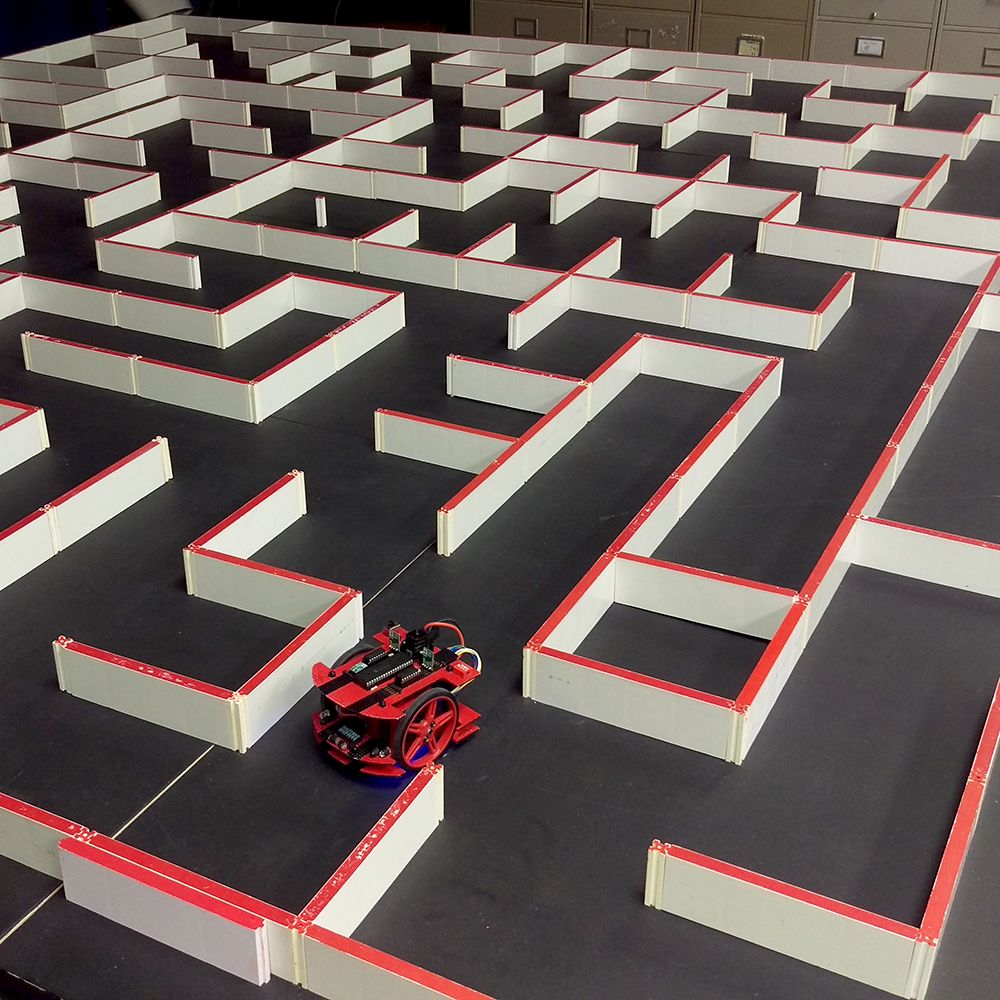
\includegraphics[width=0.6\textwidth]{figures/micromouse-maze.jpg}
    \caption{Micromouse competition photo: labyrinth and robot example \cite{MicromousePhotoLink}}
    \label{fig:micromouse}
\end{figure}

\subsection{Aims and Objectives}

    Short summary of the general competition rules is as following \cite{MicromouseRules}:

\begin{itemize}
    \item Self-Containment: A Micromouse shall be self-contained (no remote controls).
    \item Method of Movement: A Micromouse shall not jump over, fly over, climb, scratch,cut, burn, mark, damage, or destroy the walls of the maze.
    \item Maze Dimensions: The maze is composed of 18cm x 18cm unit squares arranged as 16 x 16 units. The walls of the units of the maze are 5 cm high and 1.2 cm thick 
    \item Multiple Paths: Multiple paths to the destination square are allowed and are to be expected. The destination square will be positioned so that a wall-hugging mouse will NOT be able to find it.
\end{itemize}
    
 In the case of our project, the aforementioned rules were used in a slightly modified way. The labyrinth is reduced in size to 8x8 units in order to fit better to the project conditions. The micromouse competition consists of 2 runs: in the first run, the robot is going through the maze and, according to arbitrary chosen algorithm, constructs the maze map; in the second run the mouse should reach the center of the maze (found in the first run) as quickly as possible, according to the composed map of the labyrinth. \\
 The main goal of the project was set to:  "get as close to the realization of the procedure described above as possible".
 The ways and approaches that were chosen to reach this goal are named and described properly in the next section.
 
 \subsection{Tools}
 
The list of tools used throughout the whole length of the project:
\begin{itemize}
    \item Microchip MPLABX - an IDE, used to set-up, configure and program a microcontroller. Used together with XC16 compiler from Microchip.
    \item MathWorks MATLAB \textcolor{red}{(did any of us except for Alex actually use it?)}
    \item Autodesk Eagle - PCB design software, used to create schematic diagrams, organize the component placement and route the PCB.
    \item Autodesk Fusion 360 -  CAD/CAM design software, used to build in 3D all parts of the casing for the robot.
\end{itemize}


\section{Conceptual design and justification of the design}

In order to set the right design goals and milestones during the semester, adequately estimate the workload and organize the working process in the most effective way, we needed to: analyze the initial design conditions and restrictions, roughly formulate the implementation blocks along with respective skill-sets of all project members and - after that - write down the most suitable working program. Both steps are described in detail below.

\subsection{Initial design conditions} \label{chap:design_cond}
The main question to answer was to grasp and implement using the knowledge we had acquired plus the logic behind the "how do we build a robot that should drive in the labyrinth and be able to make intelligent decisions (turns) based on the observations (made by sensors)"?

\noindent 
There are some predefined conditions and tools that we used as a starting point in answering this question: 

\begin{itemize}
    \item Geometric constraints\\ 
    As was mentioned in the previous section, the geometric parameters of the maze in our case were as following: 8x8 identical squares with a side of 16cm. Therefore, our "mouse" was logically required to be smaller than 16cm in width and length, ideally the size that would allow it to move freely while performing any type of movement within the maze (therefore leaving at least 2-3 centimeters of distance to the surrounding walls)
    \item Power supply\\
    According to the unified formal requirements of the Micromouse competition, the robot should be autonomous, which infers carrying it's own power supply in form of a standard 9V battery.
    \item Sensing the environment\\
    The initial condition in regards to sensing simply states that the robot should be able to perceive the environment and make informed decisions about the next movement (moving straight or turning in one of the directions - the turn angle was set to be fixed at 90 degrees in order to simplify the design) based on the analysis of the information received from the sensors. The sensor type that is the most efficient for the cause - simple infrared proximity sensor. We had an option to either order the desired amount of sensors or to build them ourselves.
    \item Motors\\
    In order for the "mouse" to move, we were provided with predefined 2619-SR-IE2-16 motors and sets of wheels of different diameter.
    \item Microcontroller\\
    Initially, for the educational purposes and in order to gain some knowledge in configuring and setting up the microcontroller to control the needed peripherals, a pair of dsPIC30F4011 microcontrollers was provided. Appropriate for the goal task microcontroller was decided to be chosen later. Overall, it had to have all required pins and interfaces, such as:\\
    - PWM outputs for the motor control\\
    - analog inputs to receive data from sensors\\
    - enough extra pins to connect peripherals (such as LEDs)\\
    - flexible and convenient pin mapping in order to satisfy the geometric constraints
    \item PCB\\
    The printed circuit board for the robot was to be designed independently, according to all the aforementioned conditions.
    \item Casing\\
    In order for all of the components (such as the board, the motors and the battery) to hold together in one single "mouse" unit, it was set that a custom casing must be designed and printed.
\end{itemize}

Based on those conditions and also tools and devices provided, we came up with the implementation plan, which can be seen in detail in the next part.

\subsection{Work program and Gantt chart}
In the below Fig. \ref{fig:gantt}, we describe our planned stages within a Gantt chart.

\begin{figure}[H]
    \centering
    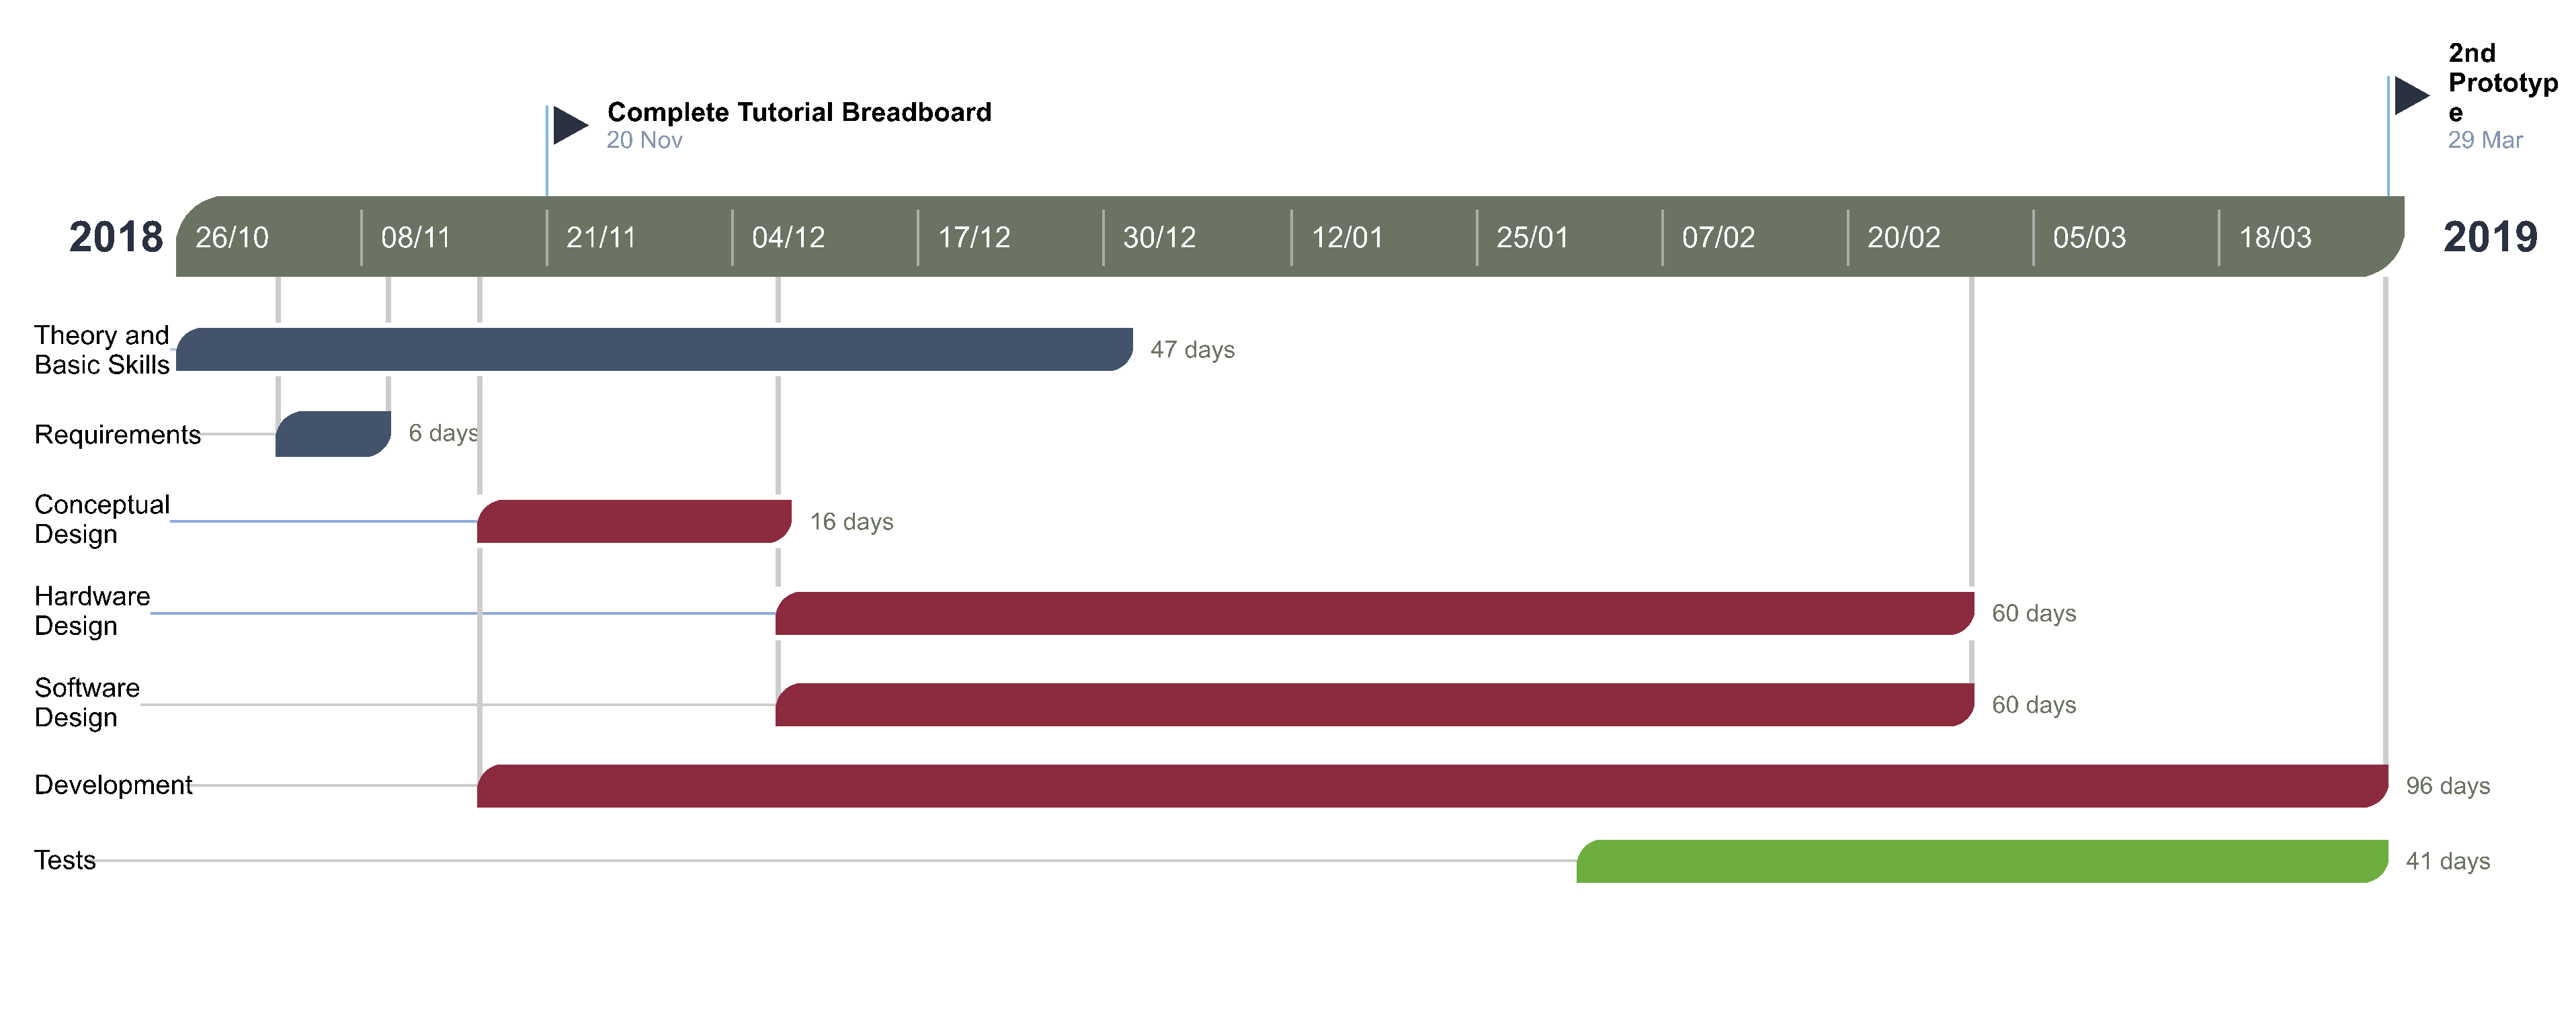
\includegraphics[width=1\textwidth]{figures/micromouse-gantt.png}
    \caption{Gantt chart of our progress}
    \label{fig:gantt}
\end{figure}

\noindent
In the first half of the semester we started off with a basic introduction to electrical engineering. By using the microcontroller dsPIC30F4012 we followed a practical course and learned to use the Microchip MPLABX environment in order to create and simulate the code for the software of the micromouse.

\noindent
The practial course was comprised of the following topics:
\begin{itemize}
    \item Digital I/O
    \item Interrupts
    \item PWM
    \item UART
    \item Quadrature Encoders
    \item Analogue Inputs
\end{itemize}

\noindent
During the practial course we applied our learnings onto a breadboard. Which can be seen in Fig. \ref{fig:breadboard}. By doing this we got an idea of what kind of electronic parts we will need to get accustomed with for the creation of the final micromouse. Our acquired knowledge will be described in more detail in the next chapter.

\begin{figure}[H]
    \centering
    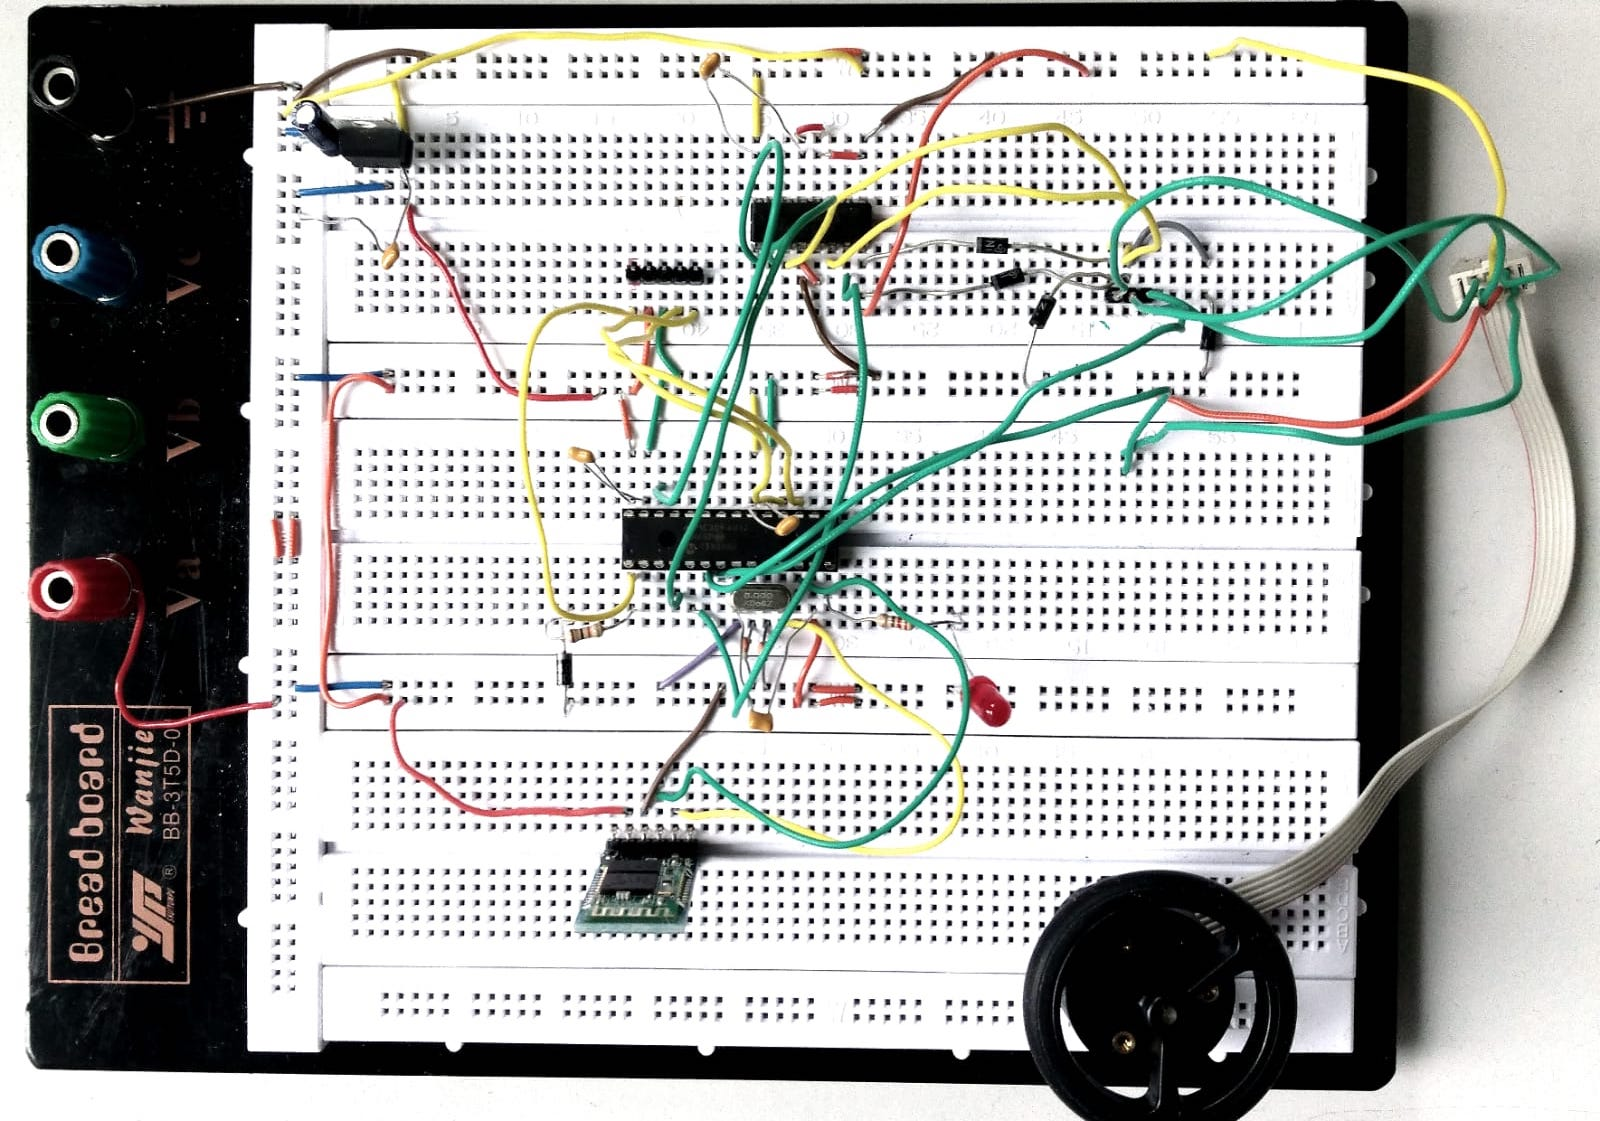
\includegraphics[width=0.6\textwidth]{figures/hardware/breadboard.jpeg}
    \caption{First completed breadboard}
    \label{fig:breadboard}
\end{figure}

\noindent
While going through the practical course, we fetched all the requirements we would need during the preparations of building the micromouse. All of them are described in the previous chapter \ref{chap:design_cond} \\

\noindent
The former idea of splitting us students into two separate groups was canceled because it took us too long to complete the basic introduction (as it was initially planned) plus the fact that we all were inexperienced in electrical engineering. Instead we formed two teams: One was responsible for the hardware the other one for the software design. This and other issues are mentioned in chapter \ref{chap:challenges}.\\
So after all requirements were known and the conceptual design phase was completed, we started with designing the hardware and software. Both are described in more detail in the chapters \ref{chap:hardware} and \ref{chap:software} respectively. \\
In order to construct a PCB with all the parts we need, we are using Autodesk Eagle. For writing the software we are using the MPLABX environment. \\

\noindent
The testing part concludes the overall development stage. But because testing is such a crucial element during a development, especially when designing hardware is a part of it, every step has to be done with caution. Hence, a failure of an electrical compound can easily lead to a broken part, which will result in unnecessary costs and time delays. The test results can be found in chapter \ref{chap:tests}. \\

\textcolor{red}{I would suggest to fit here the part with "design decisions based on the aforementioned conditions (justification)"
\textit{ This is where I'm a bit lost. We could include some "ideal" version of this chart here, but where exactly should we describe all the changes in planning and organization and why they had to be done at each stage of building the prototype and the final version of the mouse?  Should it be described here? Or later in the "problems and challenges"?
Also I think maybe here we should talk about all the initial learning stage we had to go through in the first half of the praktikum (maybe devote a subsection for this here or later in the report)}}


\section{Learning}
\noindent
The first part of the practical course was dedicated to learning the main control practices and hardware features of the dsPIC digital signal controllers from Microchip, widely used in embedded applications and robotics.\\

\noindent
\textbf{Developed skills}
\begin{itemize}
    \item extracting relevant information from datasheets
    \item expressing it in C language
    \item cross-compiling
    \item debugging (using Simulation environment)
\end{itemize}

\noindent
In the following section we introduce the most important aspects of each hardware peripheral of the microcontroller. For more details refer to dsPIC overview document \cite{alex}.\\
Please refer to the software section of the report to have more details about the peripheral’s settings used for our robot.

\subsection{Digital I/O}

The general purpose I/O (GPIO) pins allow the microcontroller to monitor and control other devices. Many pins are shared between several peripherals and the GPIO pins. An output multiplexer allows the peripheral to direct its outputs to the pin when the peripheral is enabled. Otherwise, the port is controlled by the I/O logic as shown in the figure \ref{fig:gpio} below.\\

\begin{figure}[H]
    \centering
    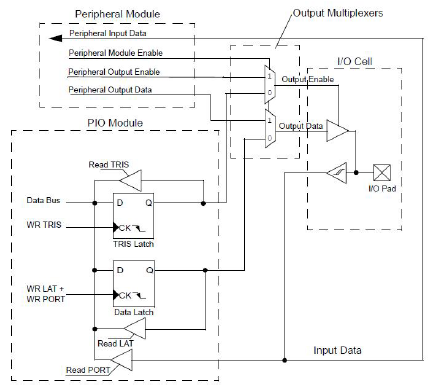
\includegraphics[width=0.5\textwidth]{figures/software/GPIO.PNG}
    \caption{Shared port structure \cite{alex}}
    \label{fig:gpio}
\end{figure}

\noindent
All port pins have three Special Function Registers (SFR), registers that control various aspects of the microprocessor's function, directly associated with the operation of the port pin:
\begin{itemize}
    \item \textbf{TRIS}\\
    The TRI-State Register sets the direction of the pin. The value ``1'' corresponds to an input pin and ``0'' to an output pin.\\
    The direction needs to be set before reading or writing the data from the ports. \\
    Only pins configured as digital can be used as input or output pins. Pins configured as analog must be used as input pin.
    \item \textbf{LAT}\\
    It sets the output value of the pin and returns the logic state of the output latch.
    \item \textbf{PORT}\\
    It returns the logic state of the pin. 
\end{itemize}
To avoid Read-Modify-Write issue, we always read from the port and write to the latch.\\

\noindent
\textit{Read-Modify-Write issue:}

\noindent
Since pins are grouped in port categories, in order to change a pin value, it is required to first load the port register in ALU, change the value with bit operations using a specific mask value and finally write the result into the port register. If there is not a long delay between two write instructions on the same port, the second operation may overwrite the first due to propagation delay. This issue is not encountered when writing on latch write since we read directly from the latch register. 

\subsection{Interrupts}

Interrupts are mechanisms that allow the microcontroller to react to external and internal events.\\
When the microcontroller receives an interrupt request (IRQ), it jumps to the interrupt service routine (ISR), executes it and returns back to the main program. 
Consequently, interrupts enable a quick reaction and are efficient for asynchronous events as they allow the microcontroller to allocate its maximum processing time for other tasks by avoiding redundant checking tasks.\\

\noindent
To be signalled to the CPU by the interrupt controller, the interrupt must be enabled and have a priority higher than the current CPU priority.\\
The natural priority is considered when two interrupts with the same assigned priority would occur simultaneously. This priority is linked to their position in the vector table.(refer to MCU datasheet table 7-1\cite{mcu})

\subsection{Timer}\label{subsec:timer}

\begin{figure}[H]
    \centering
    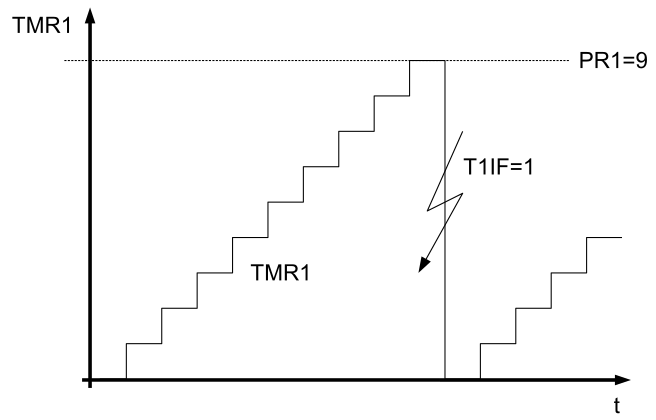
\includegraphics[width=0.5\textwidth]{figures/software/t1_demo.png}
    \caption{Principle of the Timer 1 \cite{alex}}
    \label{fig:t1_demo}
\end{figure}

Timers are used to measure the time or generate the accurate time delay using a binary counter that can be configured to count clock pulses. As seen in figure \ref{fig:t1_demo}, once it reaches the maximum set value, it rolls back to zero setting up an overflow flag and generates the interrupt if enabled. \\

\noindent
To generate the range of delays, we must set the maximum count value using the following formulas:\\
We first multiply the cycle period by a prescaler, to deduce the time between two increments of the counter:
$$tick=prescaler*T_{CY}$$
Then we derive the maxcount which we store inside our period register (PR):
$$maxcount=Timer delay/tick$$

\noindent
If we did not use a prescaler, the maximum time we could set between T1 interrupts would be $T_{CY}*(2^{16}-1)$. But since we can use a prescaler, we only count for example every second or fourth clock cycle depending on our prescaler. This allows us to wait twice or four times the amount of time.

Depending on our application, we choose a different prescaler:
\begin{enumerate}
    \item If we need a high timer resolution, the smallest prescaler value should be chosen. 
    \item If we do not care about the resolution, the highest prescaler value should be chosen. Errors in the time period relative to the period itself would be smaller with a longer period (in our case: a larger prescaler causes a longer period).
\end{enumerate}

\subsection{Pulse Width Modulation} 

\noindent
Pulse width modulation (PWM) is the method of choice to control the amount of energy that is supplied to an actuator, light source or any other device when employing digital control systems.\\
The duty cycle is defined as the proportion of time the PWM output is switched on with respect to the PWM period.
The PWM period ($T_{PWM}$) is fixed and represents the cycle time of the signal.

\noindent
As seen in figure \ref{fig:pwm_demo}, we can vary the duty cycle by changing the time that the PWM output is switched on ($T_{DC}$).

$$DC = \frac{T_{DC}}{T_{PWM}}$$

\begin{figure}[H]
    \centering
    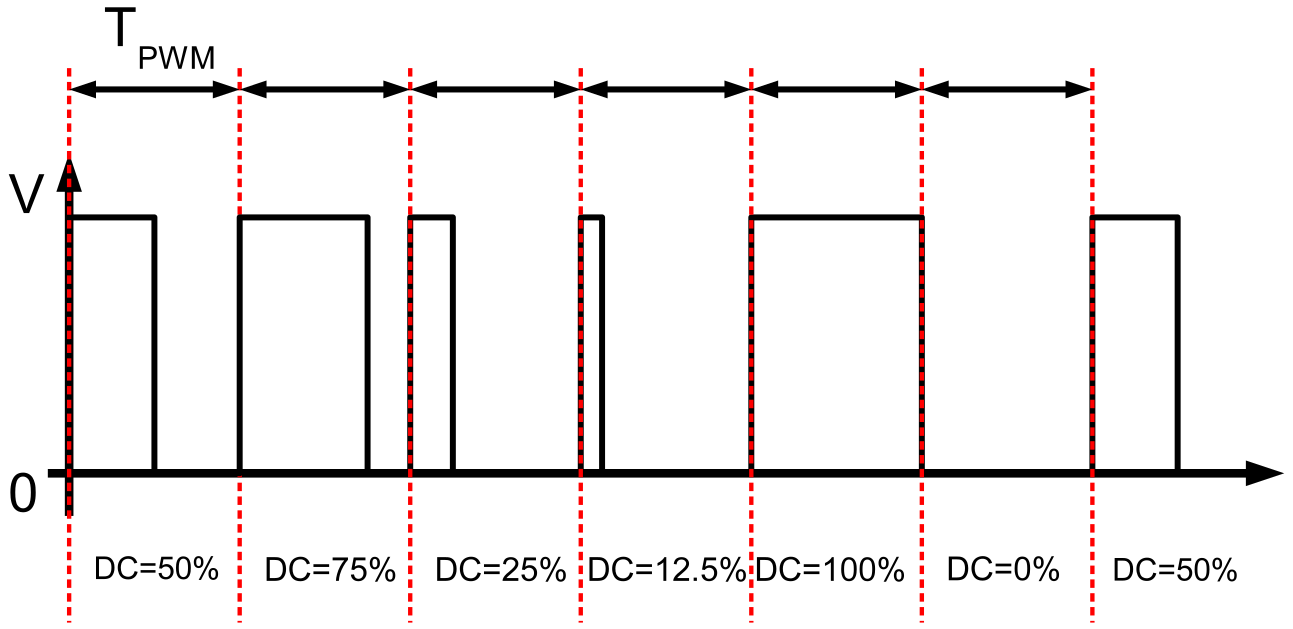
\includegraphics[width=0.5\textwidth]{figures/software/pwm_demo.png}
    \caption{Principle of PWM \cite{alex}}
    \label{fig:pwm_demo}
\end{figure}

\begin{figure}[H]
    \centering
    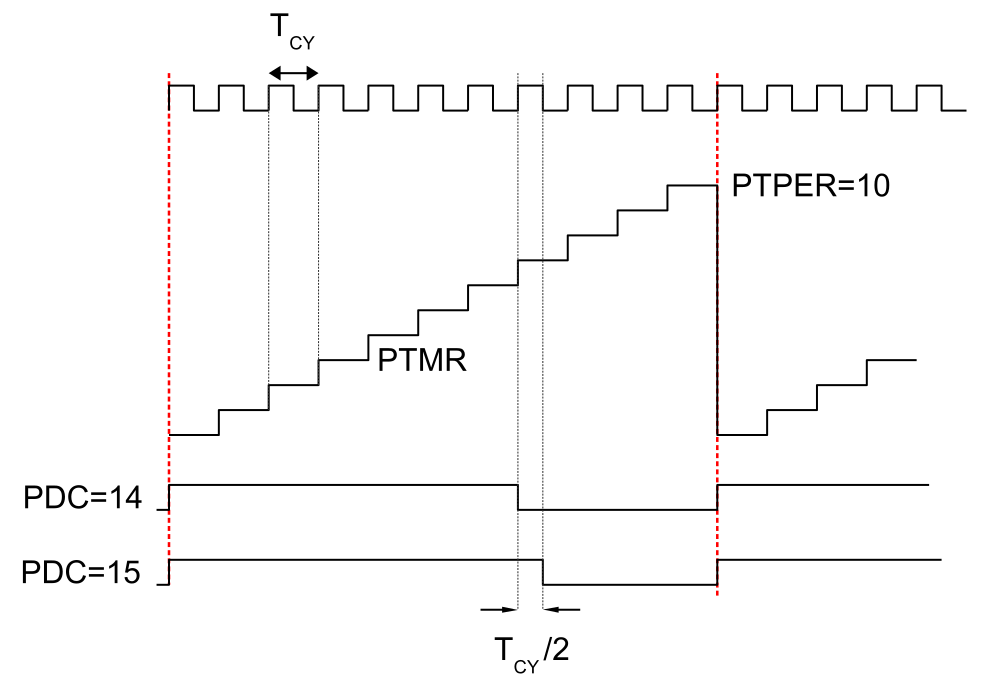
\includegraphics[width=0.5\textwidth]{figures/software/pwm_choice.png}
     \caption{Resolution of a PWM duty cycle \cite{alex}}
    \label{fig:pwm_choice}
\end{figure}

\noindent
The PWM frequency is application dependent. However, we should keep in mind that high frequency requires very fast switches and may cause electromagnetic interference problems. Whereas, low frequency causes the load to follow the pulse.\\
For driving a motor, a typical value would range between 5kHz and 50kHz, but for an accurate value we should consider the mechanical time constant and the electrical time constant of the motor.


The main elements of a PWM generator are a timer/counter and a comparator whose output drives the PWM signal. At the beginning of the cycle, the PWM signal is switched on. The comparator compares the timer/counter value with the duty cycle value ($PDC$). When this value is reached, the PWM output is switched off. The counter continues to increase until it reaches the PWM period value ($PTPER$) and then resets, completing one PWM period (see figure \ref{fig:pwm_choice}).

PWM period:
$$T_{PWM}=T_{CY}*(PTPER+1)*PTMR Prescale Value$$

DC: 
$$DC=100* \frac{PDC}{(2*(PTPER+1)}$$


\subsection{Universal Asynchronous Receiver Transmitter}

UART is the most commonly used protocol for asynchronous serial communication in microcontrollers due to its simplicity, easy implementation and minimum hardware requirements.\\

\begin{figure}[H]
    \centering
    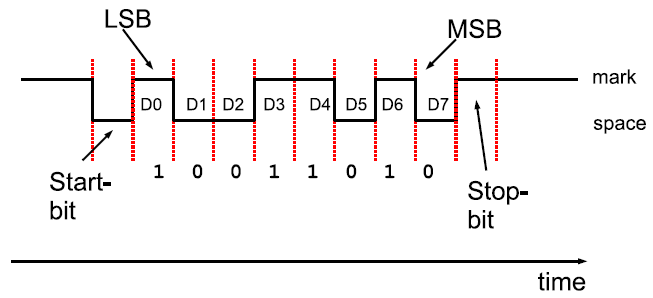
\includegraphics[width=0.5\textwidth]{figures/software/UART_com.PNG}
    \caption{UART transmission protocol\cite{alex}}
    \label{fig:uartProtocol}
\end{figure}

\noindent
As shown in figure \ref{fig:uartProtocol}, when no character is transmitted, the bus is typically logically high and transmission begins with the start bit which is logically low. After this, typically 8 data bits are transmitted and the transmission finishes with a logical high as a stop bit.\\

\noindent
To receive data from UART, we utilize a UART receive interrupt that will trigger every time a data packet is received in the UART receive registers (U1RXREG). This data is transferred to another variable and the receive buffer is cleared if full.


\noindent
The main criterion for UART communication is its baud rate, i.e. transmission speed. It is measured in bits per second and usually takes the following values: 9600bits/s, 28.8kbits/s, 57.6kbits/s.
This value is stored in U1/2BRG register and is derived from the clock cycle.
$$BaudRate = \frac{f_{CY}}{UnBRG+1}$$
For successful communication, both the device’s receiver and transmitter should be set to same baud rate.


\subsection{Quadrature Encoder Interface}

Quadrature encoders (also known as incremental encoders or optical encoders) are used for position and speed detection of rotating motion systems. They enable closed loop control of many motor control applications.
\vskip 0.2in
\noindent
The Quadrature Encoder module provides a simple interface to incremental optical encoders, which allows to obtain signed velocity using two photo-transistors that are offset by one quarter of the cycle period. It accepts the A, B and index connections from the incremental encoder and stores the accumulated count pulses in a dedicated 16-bit time base.

\begin{figure}[H]
    \centering
    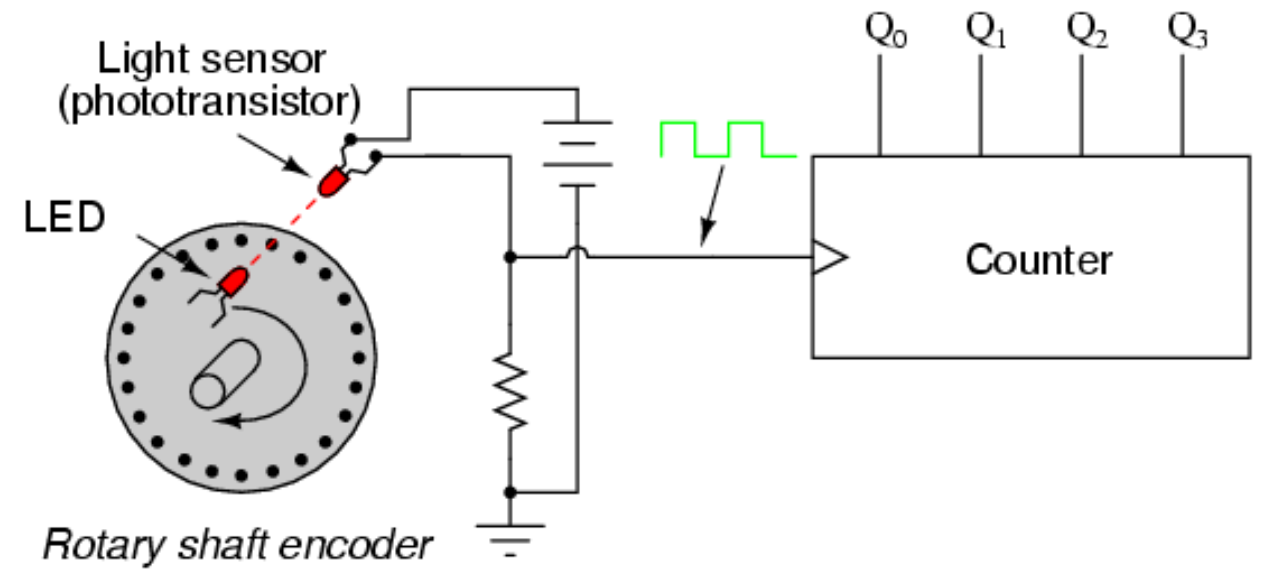
\includegraphics[width=0.5\textwidth]{figures/software/qei_demo.png}
    \caption{Principle of a Quadrature Encoder \cite{alex}}
    \label{fig:qei_demo}
\end{figure}
\vskip 0.2in
\noindent
Whenever the wheel is rotated, light emitted from the LED will hit the photo-transistor if there is a hole between them. Light sensor and emitter are separated by the wheel seen in figure \ref{fig:qei_demo}. The time passed between the phototransistor turning on after registering light and turning off again after the light disappears behind the wheel, will determine the velocity of our motor.
\vskip 0.2in
\noindent
The two channels, Phase A (QEA) and Phase B (QEB) enable to know the direction of the motor. If Phase A leads Phase B, then the direction of the motor is forward (counter is incremented). If Phase A lags Phase B then the direction of the motor is reverse (counter is decremented). A third channel, termed Index pulse, occurs once per revolution and is used as a reference to establish an absolute position.\\
However, the high resolution of the encoders leads rapidly to an overflow or underflow of the 16 bits counter register. To keep track of the total counts, a global variable should be updated accordingly at each interrupt call.

\subsection{Analog to Digital Converter}

Since we employ a digital microcontroller, it is necessary to convert the analog values from sensors to digital values. This is performed by the analog-to digital converters (ADC).\\
The ADC module converts a continuous time and value signal to a discrete time and value signal by sampling at a fixed sample period and converting the analog values into an integer values stored in a k-bits binary representation.

\vskip 0.2in
\noindent
During conversion the analog signal should be ``held'' constant throughout the process. This is usually done with a sample and hold circuit. It takes a ``snapshot'' of the input signal and stores it on the plates of a capacitor to have a steady signal. The acquisition time should be long enough for the capacitor to charge enough to match, as closely as possible, the incoming voltage.
\vskip 0.2in
\noindent
After the analog input is captured by the sample-and-hold (S/H) amplifier, it is compared with the output of a digital-to-analog converter to perform the conversion. refer to figure \ref{fig:sac} 
\vskip 0.2in
\noindent
DSPs have integrated ADCs, depending on the dsPIC type, they are either 10 bit or 12 bit ADCs.  The most commonly used ADCs are based on the successive approximation principle which uses a binary search to find each bit of the output voltage.\\

\begin{figure}[H]
    \centering
    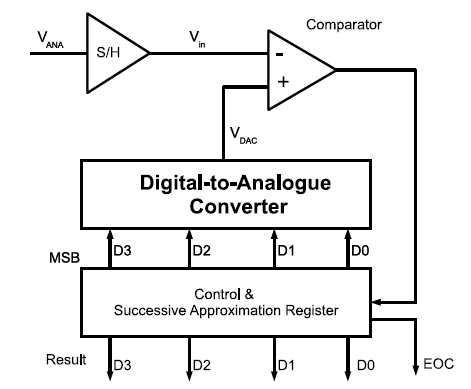
\includegraphics[width=0.5\textwidth]{figures/software/SAC.PNG}
    \caption{Successive Approximation Conversion principle\cite{alex}}
    \label{fig:sac}
\end{figure}
\noindent
ADC raises an interrupt when all the configured channels have been sampled. The results are available on the 16 16-bit ADC buffers (ADCBUF0, …, ADCUFF).


\subsection{Direct Memory Access}

Direct memory access (DMA) is the ability for an I/O device to transfer data directly to or from memory.  It can be seen as a co-processor that is used to quickly transfer data between main memory and peripherals without the intervention of the CPU. Hence, freeing up the CPU for more valuable tasks while the DMA controller takes care of the data movement and pointer incrementing.


\vskip 0.2in
\noindent
The dsPIC33 family has an integrated DMA controller optimized for high-performance, real-time, embedded applications. DMA uses a second bus master within the system and therefore, can continue to transfer data when the CPU has entered Idle mode.\\
When data is ready to be transferred from the peripheral, a DMA request is issued by the peripheral. When the block transfer is complete, the DMA channel issues an interrupt (if enabled).
\vskip 0.2in
\noindent
The DMA channel supports different operating modes:
\begin{itemize}
    \item Post-Increment or static DPSRAM addressing.
    \item Peripheral Indirect Addressing or Register Indirect Addressing.
    \item One-Shot or continuous block transfers.
    \item Ping-Pong mode (Auto-switch between two start addresses offsets (DMAxSTA or DMAxSTB) after each transfer complete)
\end{itemize}

\noindent
Please refer to the DMA section of the Family reference manual \cite{dma} for more details about these operating modes.


\subsection{Fusion Workshop}
For learning Autodesk Fusion 360, a one-day workshop was held. In this workshop, the basic aspects of CAD modelling and basic features of Fusion 360 were introduced, as well as more advanced features such as history timeline, version control, and collaboration between users.

One very helpful thing that we learned in the workshop is to import 3rd party parts. The 3D model of the motor that we are using is imported, such that a fitting motor mount can be designed very precisely and accurately according to the dimension of the motor. (Fig. \ref{fig:fusion_import})

We practiced using many “modeling” features, as well as “assembly” features such as joint, and changing “physical material” and “appearance” to create a box with a moving joint that can be opened and has varying appearances. Later the user collaboration feature was demonstrated using these boxes by assembling them on a table. (Fig. \ref{fig:fusion_collab_table})

\begin{figure}[htb]
    \centering
    \begin{minipage}{.45\textwidth}
          \centering
            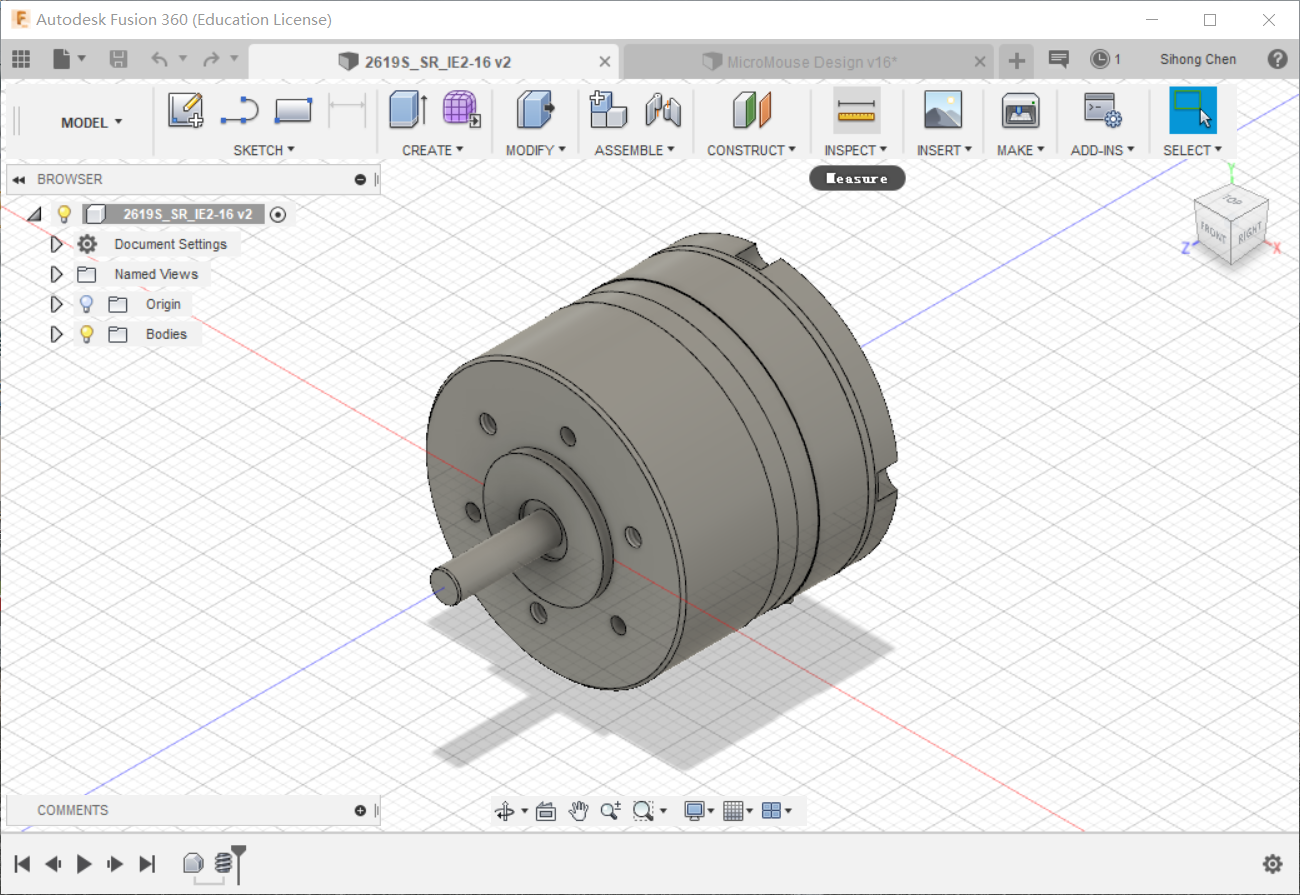
\includegraphics[width=.9\linewidth]{figures/Casing/FusionImport.PNG}
              \caption{Import 3D CAD Model from 3rd party}
                \label{fig:fusion_import}
    \end{minipage}
    \begin{minipage}{.45\textwidth}
          \centering
            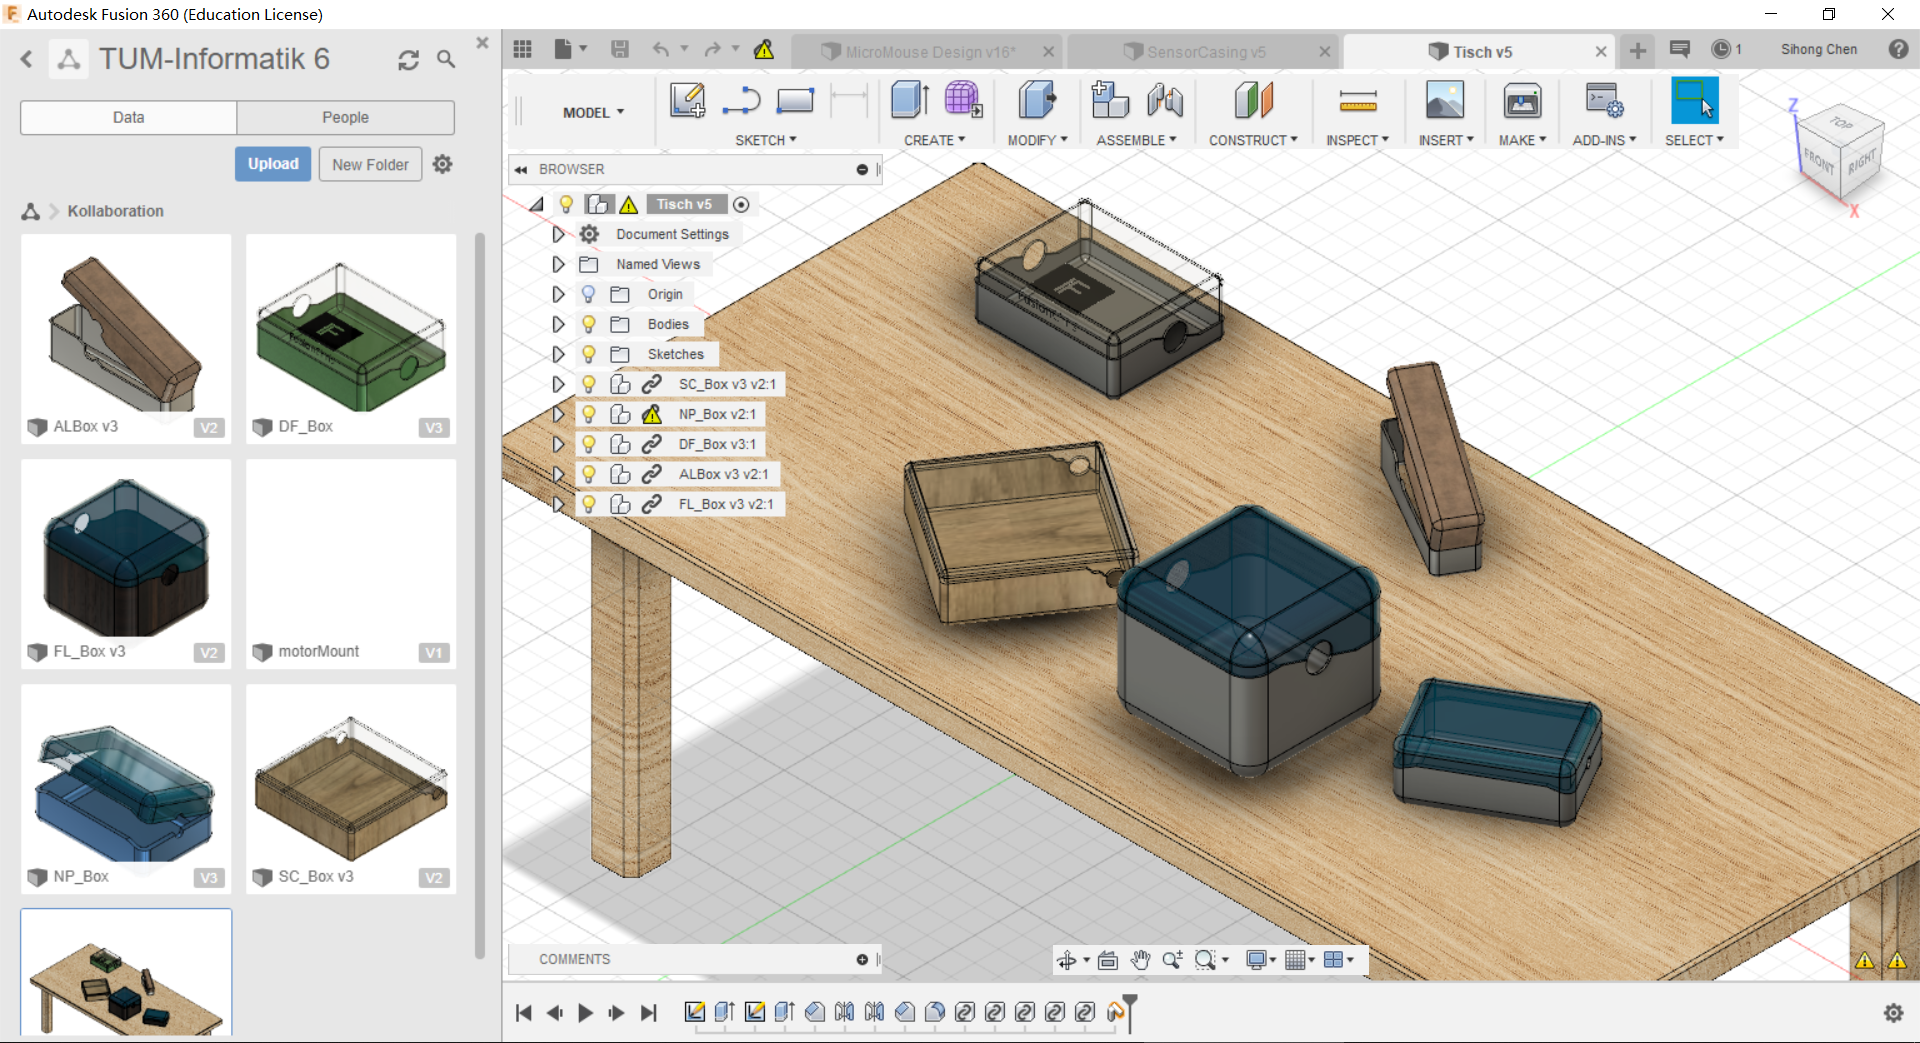
\includegraphics[width=.9\linewidth]{figures/Casing/FusionCollaborationTable.PNG}
              \caption{Individually made boxes put together on one table in Fusion collaboration}
                \label{fig:fusion_collab_table}
    \end{minipage}
\end{figure}

\noindent
In the workshop, a synchronisation feature between Autodesk EAGLE and Autodesk Fusion 360 is briefly introduced, which has the potential to reduce the back-and-forth process between CAD 3D model design and PCB design. However, in practice, we find that the lack of 3D models from the electronic components that we are using renders the usefulness of this feature somewhat limited.

In order to tackle some of the challenges we faced for designing the casing, some more advanced features of Fusion 360 have been utilised.

\noindent
One example is to set “parameter” values when creating the parts, which allowed easy modification to the model. This is helpful because our design processes are parallel to each other, and in the end the casing has to matched the physical dimension of the board. Therefore a back-and-forth process between PCB design and CAD design is unavoidable. The “parameter” feature in Fusion 360 accelerates this process and saves a lot of time and unnecessary work.

Furthermore the freeform and sculpting tool enables us to create more free flowing surfaces. This tool is traditionally reserved for industrial designers, and by combining this with the CAD solid modelling environment, Fusion 360 has partially earned its namesake: a fusion of different design processes. For our project, it enabled a more interesting look to the design.

\FloatBarrier
\vspace{1cm}



\section{Hardware design} \label{chap:hardware}

In this section, the hardware design and implementation of the micromouse robot are described. First, the corresponding electrical circuit, known as Schematic, is broken down to its components and thoroughly presented. In the next subsection, the actual components chosen for the hardware implementation are listed. The model for the final Printed Circuit Board (PCB) follows right after. Last, but not least, the protective casing for the micromouse is described.

\vspace{1cm}

\subsection{Schematic and Components Description}

The first step in the development of the hardware is the drawing of the electrical circuit. The realization of a moving micromouse demands for the combination of a variety of components connected to each other. Exactly this is described in the so called Schematic of the circuit, which resembles a drawing on paper. 
The Schematic of the micromouse can be seen in Fig. \ref{fig:schematic_overview}.

\begin{figure}[H]
    \centering
    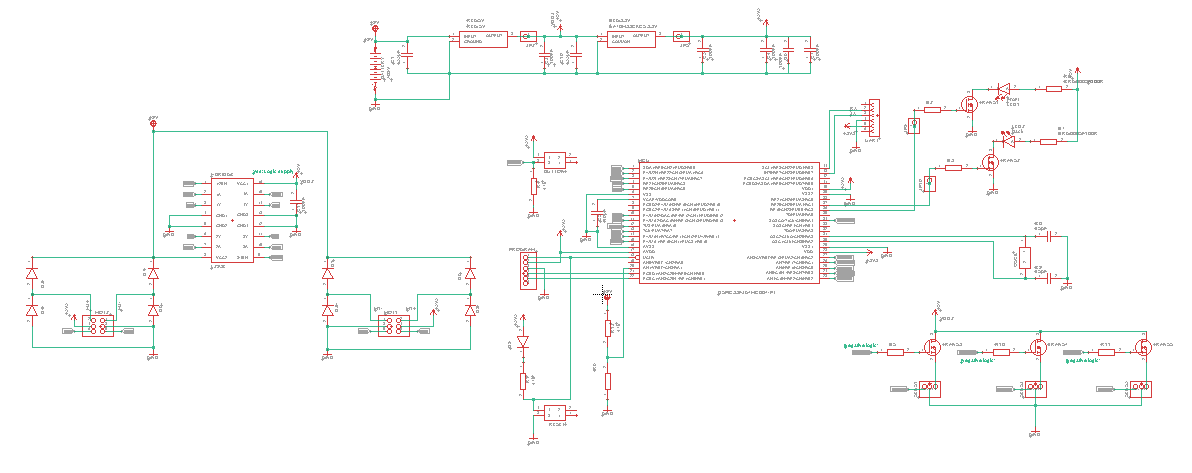
\includegraphics[width=1\textwidth]{figures/hardware/Schematic.PNG}
    \caption{Schematic overview of the micromouse}
    \label{fig:schematic_overview}
\end{figure}

\noindent
This can look intimidating at first and definitely not readable in such a miniature picture. So, let's break it down to its components and describe its sub-circuits. Notice that all of the components appearing in the Schematic were downloaded one by one from the suppliers' site, together with their PCB models, as will be seen later.

With the exception of the first subsection, the components will be presented from left to right and from top to bottom, so that the reader may always refer to the overview schematic to get a clear picture of a component's relation to the whole.

\FloatBarrier
\vspace{1cm}

\subsubsection{Microcontroller (MCU)}

The microcontroller (mcu) can be seen in Fig. \ref{fig:mcuL}.
Notice that the symbolic representation of the mcu, specifically when it comes to the location of its pins, doesn't correspond to the real model. For the purpose of the schematic, we don't really care about the real location of the pins. As will be seen later, this becomes of importance when placing the components on the board to be printed.

\begin{figure}[htb]
    \centering
    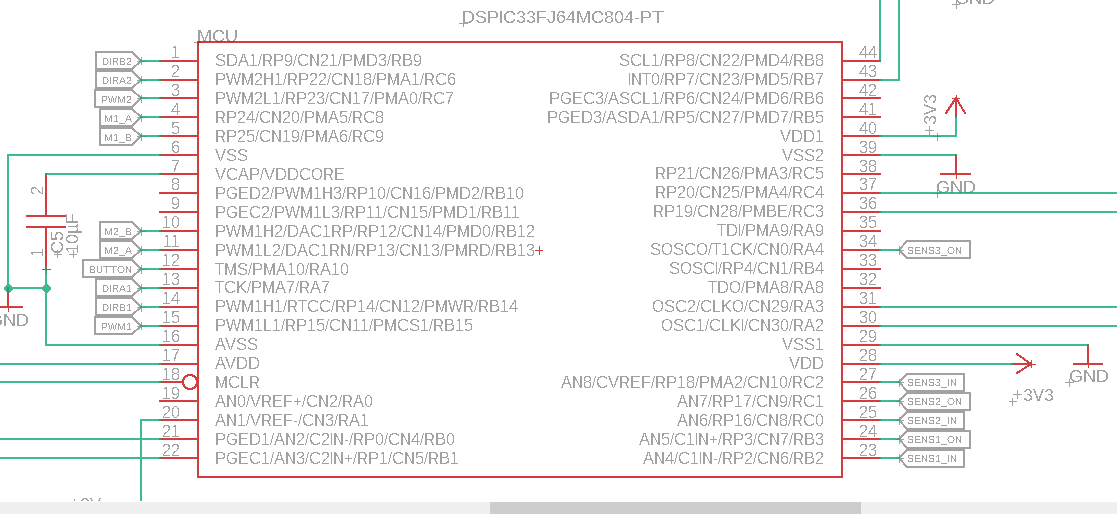
\includegraphics[width=1\textwidth]{figures/hardware/MCU.PNG}
    \caption{The dsPIC33FJ64MC804 microcontroller}
    \label{fig:mcuL}
\end{figure}

\FloatBarrier

\noindent
The assignment of mcu pins to components is presented in the software section and will not be repeated here. Please refer to that section for understanding the functionality of its pins in our circuit.

Another point to notice about the pin connections is the convenient label feature that Autodesk Eagle offers. Notice how some of the components are wired to the pins of the mcu, while other connections are represented as labels. Labels in the circuit are the equivalent of wires and greatly contribute to the readability and modularity of the schematic. As long as two wires anywhere in the circuit share the same label, they are connected.

A last comment has to be made about the pins of the mcu: The pins, as everything in our circuit, are very real components and therefore are subject to electrical limitations. This is a very important point to keep in mind, when driving any load, such as LEDs or a motor, but also when connecting input signals, such as sensors.
Specifically, in the section "Electrical Characteristics" in the mcu datasheet \cite{mcu}, we find maximum values for individual pins and for all utilized pins combined. These can be seen in Fig. \ref{fig:electrical}. These characteristics lead to some important design decisions, specifically named in later subsections.

\begin{figure}[htb]
    \centering
    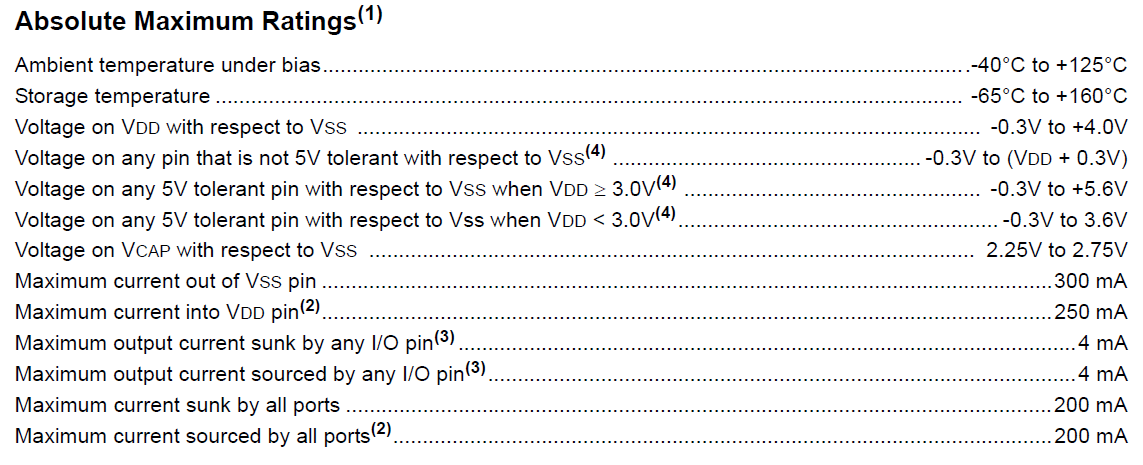
\includegraphics[width=0.8\textwidth]{figures/hardware/Electrical.PNG}
    \caption{Electrical limitations for the pins of the mcu}
    \label{fig:electrical}
\end{figure}

\FloatBarrier
\vspace{1cm}

\subsubsection{Voltage Regulators}

The necessity for voltage regulators, which can be seen in Fig. \ref{fig:battery}, arises from the need for different voltages present in our system. 
Specifically, as found in \cite{mcu}, the mcu considers 3.3V as logical one and it is this voltage we need to provide to it (see $V_{DD}$ pins). The distance sensors used (taken from a previous micromouse model) need 5V. And yet the motors need 6V, as can be seen in \cite{motor}. 
Notice that we are using a battery of 9V. Therefore, we need a way to generate the required three different voltages.

\begin{figure}[htb]
    \centering
    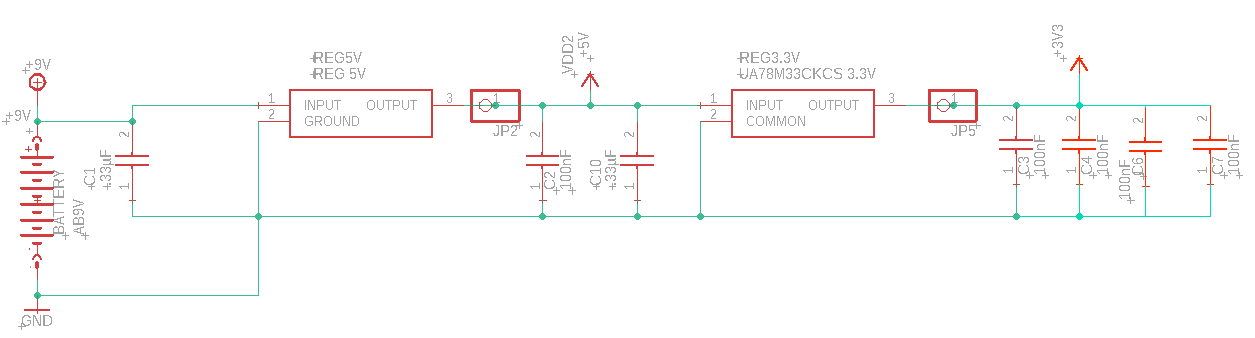
\includegraphics[width=1\textwidth]{figures/hardware/VoltageandCapacitors.PNG}
    \caption{The battery and voltage regulators}
    \label{fig:battery}
\end{figure}

\FloatBarrier

When it comes to the motor, we can regulate the voltage we feed it with, by regulating the maximum duty cycle of the PWM (explained in another section). So, we provide it with a fraction of the available 9V.
For the distance sensors and the mcu, two voltage regulators are used in succession. They provide our components with steady voltage, necessary for functioning properly. A voltage regulator essentially contains a variable resistor, which changes according to current needs of the load, e.g. the mcu, in order to provide a stable voltage in its output.

A question that arises is: Why use 9V, when much less is actually needed in the circuit? One needs to keep in mind that voltage regulators need a minimum difference between the input and the output voltage to ensure steady output voltage. This difference is called "dropout voltage" and can be found in the datasheets of the voltage regulators \cite{3.3V}, \cite{5V}. For example, the dropout voltage of both the regulators we have chosen for our micromouse is 2V. So, one sees that provision for higher extra voltage has to be made.

Now, notice the capacitors used in Fig. \ref{fig:battery}. Capacitors are used in the input and output of the voltage regulators. As can be read in the datasheets of the regulators \cite{3.3V}, \cite{5V}, the capacitors' values are well specified and they are required for the behavior of the regulators to be optimal. Specifically, the input capacitor functions as noise filtering for the voltage supply and the output one ensures improved transient response. For a deeper understanding on the transient response of regulators, refer to \cite{regul}. The article refers to low-dropout linear regulators (it"s not the case for the voltage regulators used here, with 2V dropout), but the main principle of the output capacitor holds just the same.

Additionally,  few capacitors can be observed at the far right part of the sub-circuit.
These capacitors have both a special name and function: They are called decoupling capacitors and their role is to help provide steady voltage and current to the load (here our mcu). Specifically, they are always physically connected close to their corresponding component and should a temporary lack of electrons happen, they provide from their surplus, keeping the voltage and current steady. Such an event can happen frequently, since the mcu is a load that changes its demands on current, depending to the components it's,  in turn, connected to. By changing the demand on current, the voltage regulator, being essentially a variable resistor, needs to readjust, in order to provide the new current. This refers to the transient response of the regulator and it takes a small amount of time for the regulator to adjust. During that time, the decoupling capacitor offers the electrons and thus the current needed.

The decoupling capacitors are only symbolically placed there in the circuit. In reality, they are connected between the pins of the mcu that connect to $V_{DD}$ (3.3V) and ground (GND). Every decoupling capacitor is ideally connected as close to the actual component pins as possible, as will be later seen in the PCB Section. The values of the capacitors are dictated by the datasheets of the specific components used. For example, have a look in \cite{mcu}.

\vspace{1cm}


\subsubsection{H-bridge and Motors}

Next, the motors and H-bridge sub-circuit will be presented. 
First, let us consider the motors. As can be seen in Fig. \ref{fig:motors}, the motors are symmetrically connected to the H-bridge and to the mcu. So, let us concentrate on one of them, the left. The same explanation applies for the other one.

\begin{figure}[htb]
    \centering
    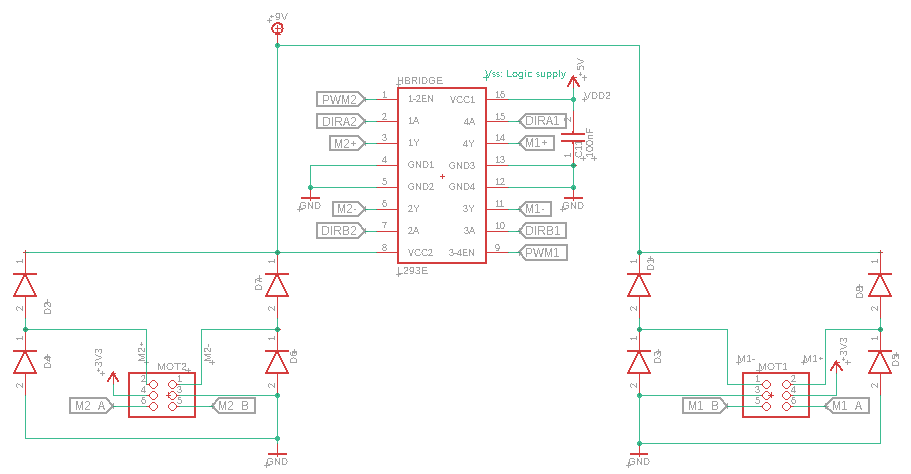
\includegraphics[width=1\textwidth]{figures/hardware/Motors.PNG}
    \caption{The motors and the H-bridge}
    \label{fig:motors}
\end{figure}

\FloatBarrier
\noindent
In Fig. \ref{fig:motorPins} taken from the motor datasheet, the motor pins can be noticed. 
One pair of pins (1, 2) refers to the voltage we feed to the motor. Remember that we are using PWM (max 6V) to control how fast the motor turns and notice that if the voltage is reversed, the rotation of the motor is also reversed. As we will shortly see, for this purpose, the H-bridge is needed. The function of reversing the motor's rotation is highgly desirable, since we want our 2-wheels micromouse to be able to move backwards and to turn on spot (imagine one wheel moving to one direction and the other to the opposite direction with the same velocity).

\begin{figure}[htb]
    \centering
    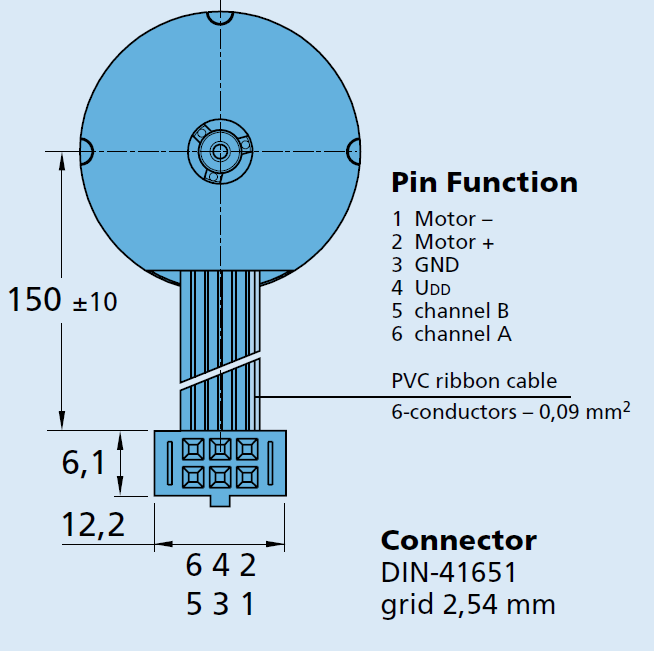
\includegraphics[width=0.8\textwidth]{figures/hardware/motor.PNG}
    \caption{The motor pins as presented in its datasheet}
    \label{fig:motorPins}
\end{figure}

\FloatBarrier
\noindent
Another pair of pins (3, 4) refers to the voltage feed of the motor encoder. And the last pair of pins (5, 6) is used for the output of the motor encoder signals. These signals encode the motor's rotational position every moment and are fed to the mcu. In the mcu, with the help of the quadrature encoder (QE) module, they can be translated to real position in space.

Finally, let us consider the H-bridge. As mentioned, the need for the H-bridge arises from the function of reversing the motor polarity and thus its rotation. Without the use of an H-bridge, one would have to physically reverse the wires for the motor feed. If it is impractical with the use of wires, it is impossible with the traces on a PCB. Instead, the H-bridge can conveniently reverse the voltage. 

The main principle of an H-bridge can be seen in Fig. \ref{fig:HPrinciple}. The bridge functions with a pair of switches (MOSFETs in the figure). When one pair is closed, current flows through the motor and it rotates to one direction. Notice that at the same time, the other set of switches is open. When we want the motor to rotate in the other direction, the other set of switches closes and this one opens. A time delay is necessary, when all switches are open, else the voltage source will be short-circuited and this is something we want to avoid at all costs.

\begin{figure}[htb]
    \centering
    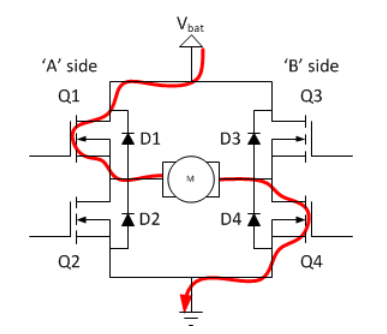
\includegraphics[width=0.8\textwidth]{figures/hardware/H-Principle.PNG}
    \caption{The principle of how an H-bridge allows flipping rotation direction of the motor, taken from \cite{catchDiodes}}
    \label{fig:HPrinciple}
\end{figure}

\noindent
Next, have a look at the exemplary circuit in Fig. \ref{fig:HData}, taken from the datasheet of the H-bridge \cite{Hbridge}.

\begin{figure}[htb]
    \centering
    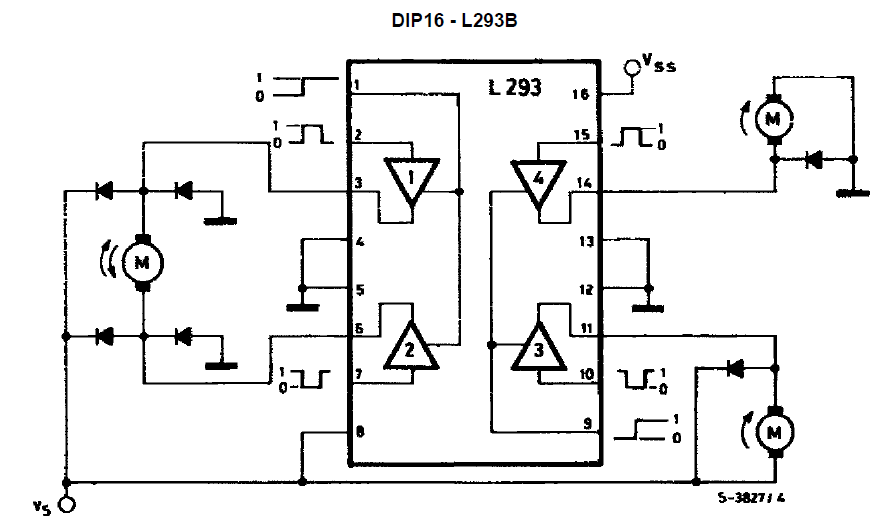
\includegraphics[width=0.8\textwidth]{figures/hardware/HbridgeDatasheet.PNG}
    \caption{Exemplary motor connection from the H-bridge datasheet}
    \label{fig:HData}
\end{figure}

\FloatBarrier
\noindent
We feed our PWM in pin 1. Pins 2 and 7 are used for controlling the direction of rotation of the motor. The truth table is simple: If one direction pin is "1" and the other "0", then the logical "1" defines the direction. If both of the pins are set to logical "0" or "1", the motor breaks. Notice how the pins 3 and 6 feed the voltage to the motor and are coupled with the direction pins. Comparing figures \ref{fig:HPrinciple} and \ref{fig:HData}, the direction pins in the latter hide inside them the functioning pair of switches mentioned in the earlier.

As a last comment, in both Fig. \ref{fig:HData} and Fig. \ref{fig:motors} notice the existence of diodes. Again, these diodes have both a special name and a special function. They are called \textit{catch diodes} and to understand their use, please refer to \cite{catchDiodes}, where a beginners-friendly introduction to H-bridges is offered.
For our purposes, it suffices to say that the presence of catch diodes is necessary for the smooth functioning of our brushed motor. Consider the case, when the motor changes direction or stops from spinning. In order for this to happen, the internal switches of the H-bridge need to open (remember the direction pins). Temporarily, the current that was flowing in the circuit through the motor has to go ("escape") somewhere, since due to the inductance nature of the motor, the current cannot instantly go to zero . It is not a good idea to dissipate the current through our H-bridge pins/ switches, without an alternative: The current will try to jump an open switch, creating a spark and probably burning the pin/switch. The catch diodes provide this alternative: The current flows through them in a forward way and is returned to the source.

\vspace{1cm}


\subsubsection{Extra Button}

Naturally, the more input options we have for our micromouse robot, the more flexible the commands we can issue and the more complicated the software can be. Therefore, we added a button (switch), which can be seen in Fig. \ref{fig:button}.

\begin{figure}[htb]
    \centering
    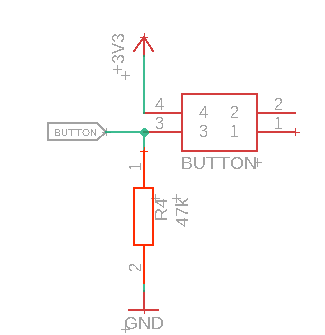
\includegraphics[width=0.8\textwidth]{figures/hardware/Button.PNG}
    \caption{An extra button for input}
    \label{fig:button}
\end{figure}

\FloatBarrier
\noindent
A typical pull-down resistor of 47k is used, to make sure the mcu pin never has an undefined logical value ("floating"). When it comes to the resistance value, it is somewhat arbitrary in that it does its job. A different value could have been selected.
For the current that flows through the resistor, when the button is pressed, we have:

$$V = I*R => 3.3 = I*47 => I = 0.07mA$$

If a much smaller value for the resistance was used, then the current would be much larger, leading to unnecessary power dissipation on the resistance and heating. Also, in this case, there is the possibility for the input to the mcu pin to be stuck in a low, logical 0 level, no matter if the button is pressed or not.

\vspace{1cm}


\subsubsection{Programmer}

The programmer is the device that allows for (re)programming of the mcu. The way it is connected is rather straightforward and can be seen in Fig. \ref{fig:programmer}.
Of particular interest is the use of the MCLR pin (Master Clear) in the mcu. In order for the EEPROM (electrically erasable programmable read-only memory) to be reprogrammed, the programmer device needs to raise the voltage of this pin higher than $V_{DD}$. The MCLR pin is used both for programming and resetting purposes.

\begin{figure}[htb]
    \centering
    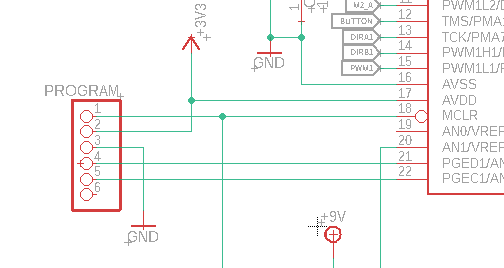
\includegraphics[width=0.8\textwidth]{figures/hardware/Programmer.PNG}
    \caption{The programmer}
    \label{fig:programmer}
\end{figure}

\noindent
More details about the reprogramming of the flash memory of the mcu can be found in \cite{mcu}, in the section "FLASH PROGRAM MEMORY".

\FloatBarrier
\vspace{1cm}


\subsubsection{Reset Button}

A reset button is needed in case something goes wrong during the execution of the program in the mcu, or if one simply needs to start the execution from the start again. Notice that the MCLR (Master Clear) pin is also used by the programmer for programming and debugging, as can be found in \cite{mcu}.

\noindent
The reset activation logic in our mcu is negative or inverse, as can be seen in Fig. \ref{fig:reset}. A diode and a pull-up resistor (similar to the pull-down used for the other button) connect the voltage feed to the mcu. Once the button is pressed, a connection with the ground is made and the mcu is reset. Remember from the previous section, that during programming of the mcu, the voltage for this particular pin is raised higher than 3.3V. For this reason, the diode is needed in series with the pull-up resistor.
Again the choice of the resistance value is a bit arbitrary.

\begin{figure}[H]
    \centering
    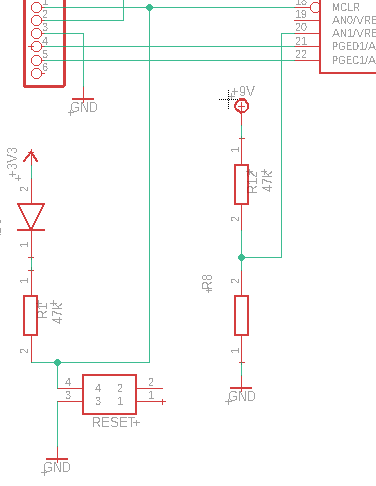
\includegraphics[width=0.8\textwidth]{figures/hardware/MCLRandBatteryMeasurement.PNG}
    \caption{The reset button and the battery voltage measurement circuit}
    \label{fig:reset}
\end{figure}

\vspace{1cm}


\subsubsection{Battery Measurement}

In an ideal world, our battery would provide steadily 9V until its exhaustion. However, this is not the case. As the battery is depleted, the voltage it provides is reduced. It would be useful to know exactly how much voltage the battery provides at any given point in time. Feeding this value to the mcu, we can take decisions accordingly. For example, we can regulate the PWM maximum duty cycle value to keep the motor spinning at its maximum velocity, even though the battery is depleted. Remember that our motor can take a maximum of 6V for its fastest performance.

Additionally, as described in the subsection \textit{Voltage Regulators} above, the voltage regulators have a characteristic dropout voltage. In this case, the 5V voltage regulator will stop providing steady 5V, once the battery starts offering less than 7V. This means, that our circuit will malfunction, from the mcu to the distance sensors. We need to detect this in time to change the battery.

In order to realize such a schema, a simple voltage divider sub-circuit and an analog pin of the mcu can be used, as can be seen in the above Fig. \ref{fig:reset}.
In order to keep the amount of different components to a minimum, a resistance of 47k is used. The question now is, what should the value of the other resistance be, in order for the input voltage to the mcu to be 3.3V for a 9V battery. 

If we call the unknown resistor $R_8$, as in the figure, we can use the known equation for a voltage divider:

$$V_{MCU} = \frac{R_8}{47+R_8} * 9V = 3.3V$$

\noindent
With a value of $ R_8 = 22k $, we can easily calculate the resulting $V_{MCU} = 2.87V$. This is a convenient value, since for example another battery of higher voltage, e.g. 10V, could be used. By choosing this value we fulfill our initial purpose and have some flexibility for higher voltages.

\FloatBarrier
\vspace{1cm}

\subsubsection{Universal Asynchronous Communication (UART)}

Despite us building an autonomous micromouse robot that can navigate in a labyrinth, we would still like to be able to issue stand-alone commands via UART. Hence, the UART sub-circuit of Fig. \ref{fig:uart}. The connection is straight-forward. Only attention is required in connecting RX to TX of the mcu and vice-versa.

\begin{figure}[htb]
    \centering
    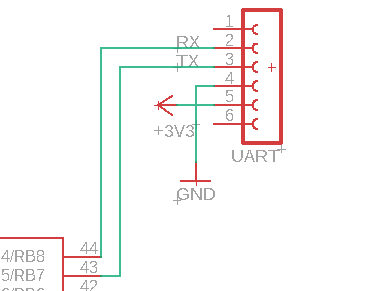
\includegraphics[width=0.8\textwidth]{figures/hardware/UART.PNG}
    \caption{The UART module}
    \label{fig:uart}
\end{figure}

\FloatBarrier
\vspace{1cm}


\subsubsection{Light-emmiting Diodes (LEDs)}

To motivate the use of two LEDs in our micromouse, imagine the following: The PCB lies on the two wheels, which are screwed on either side somewhere in the middle. Naturally, the PCB will tilt forwards or backwards until it touches the ground, depending on where most weight lies (front sensors). This is highly unwanted: Not only would it result in an unelegant movement creating uneccessary impedance, but the PCB could be potentially damaged by friction and by ground anomalies.

Therefore, for mechanical stability, we use one LED on the front and one on the back of our PCB. They are through-hole components, with the head of the LED resting on the under side of the PCB. The smooth surface of the head works to our favor, not only stabilizing the micromouse, but also offering minimum resistance while moving. The height of the protruding LED head can be decided during soldering according to mechanical needs.

Now, since we have the LEDs, it would be nice to be able to turn them on and off at will. For example we can light the front LED when the micromouse is moving forward and the back one when it's moving backwards.
The sub-circuit for controlling the LEDs can be seen in Fig. \ref{fig:leds}.

\begin{figure}[htb]
    \centering
    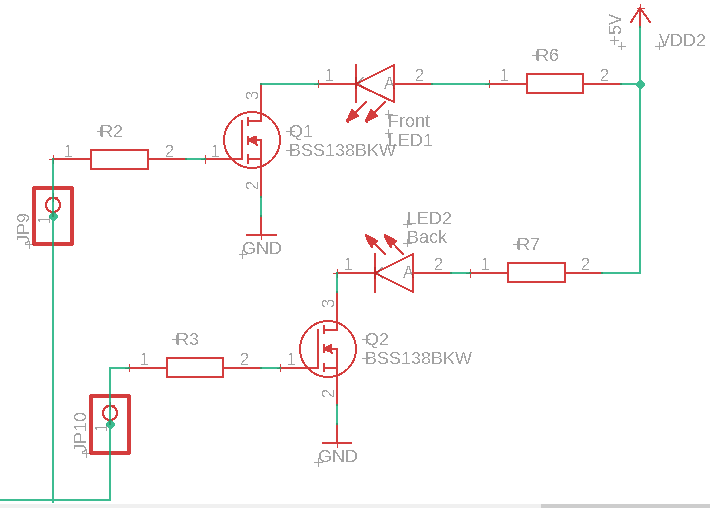
\includegraphics[width=0.8\textwidth]{figures/hardware/LEDs.PNG}
    \caption{The LEDs used for mechanical stability}
    \label{fig:leds}
\end{figure}

\FloatBarrier
\noindent
The sub-circuits for both LEDs are identical, so let us examine one of them, say the front one. The main component, besides the LED, is an N-channel metal-oxide semiconductor field-effect transistor (MOSFET).

To motivate the need for the MOSFET, imagine connecting the LED directly to the I/O pin. In the datasheet of a typical low current LED (and also the one we will be using) \cite{leds}, we find that the current can be somewhere between 25 to 140 mA. However, the value of 140mA can only be reached under certain PWM conditions. In our case, 20mA steady current will suffice for a bright enough LED. Also the voltage drop on the LED is 2.2 to 2.5V for $I = 20mA$.

Remember the electrical characteristics of the mcu pins as presented in Fig. \ref{fig:electrical}. Notice that the limit current per pin is 4mA! In other words, if we directly connect the LED to the mcu, we will damage the mcu pin and potentially other parts of the mcu circuit. 
Now, the MOSFET serves as a switch: By providing a low current to its gate (the pin of the MOSFET connected to the mcu pin), its channel between the drain and source opens. In other words, it allows current to flow from the LED side to the ground side, thus closing the circuit and lighting the LED up! 

The resistor R2 in the sub-circuit is used to charge the capacitance of the transistor gate. Hence its value is not critical in our case, since no intense time precision demands are made on the LED. We can use our typical 47k resistors also here. Notice that exactly next to the mcu pin, a header pin is placed with the name JP9. This is just a convenient way to later check the voltage of the pin on the PCB for debugging purposes.


The last component to cover is the resistor on the side of the LED. To choose an appropriate value, we need to consider the voltage drop on the LED. As we read above it's somewhere between 2.2 and 2.5V. We can use $\Omega$hm's law, by considering the resistance of the transistor negligible and the resistance of the diode fixed. For the current flowing, let's choose 20mA as stated above. 

$$V_R = I * R => 5 - V_{diode} = I * R$$

For the values $V_{diode} = 2.2V$ and $I = 20mA$ we acquire a value of 140$\Omega$. So, this is the value we need for the resistor.

\vspace{1cm}

\subsubsection{Oscillator}

The external oscillator and its capacitors can be seen in Fig. \ref{fig:oscillator}. As can be found in the datasheet of the mcu \cite{mcu}, the internal oscillator offers up to 8MHz frequency. For this reason and also for the flexibility of being able to choose, we opted out for a 16Mhz external oscillator.
The capacitors are necessary for the functioning of the crystal oscillator, since they are not included in it.

\begin{figure}[htb]
    \centering
    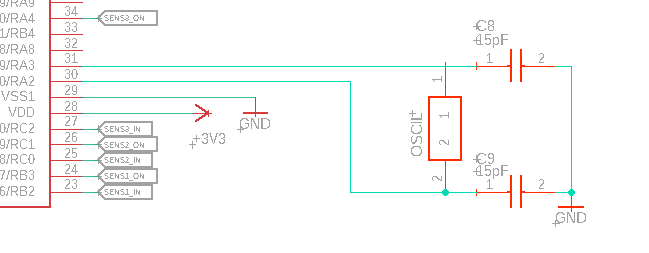
\includegraphics[width=0.8\textwidth]{figures/hardware/Oscillator.PNG}
    \caption{The external oscillator}
    \label{fig:oscillator}
\end{figure}

\FloatBarrier
\vspace{1cm}


\subsubsection{Distance Sensors}

The distance sensors are necessary for perceiving the distance from maze walls. Their sub-circuit can be seen in Fig. \ref{fig:sensors}.

\begin{figure}[htb]
    \centering
    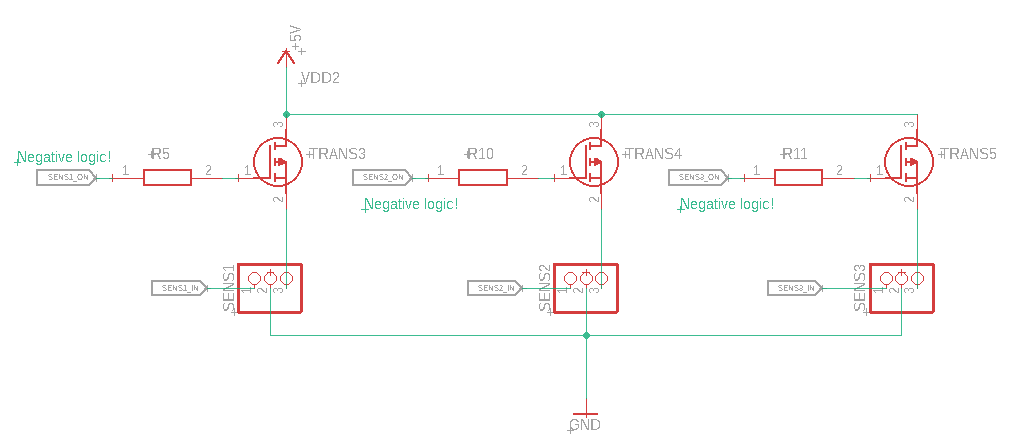
\includegraphics[width=1\textwidth]{figures/hardware/DistanceSensors.PNG}
    \caption{The distance sensors}
    \label{fig:sensors}
\end{figure}

\FloatBarrier
\noindent
To understand their pins, have a look at Fig. \ref{fig:sensorsData} taken from the datasheet \cite{sens}.

\begin{figure}[htb]
    \centering
    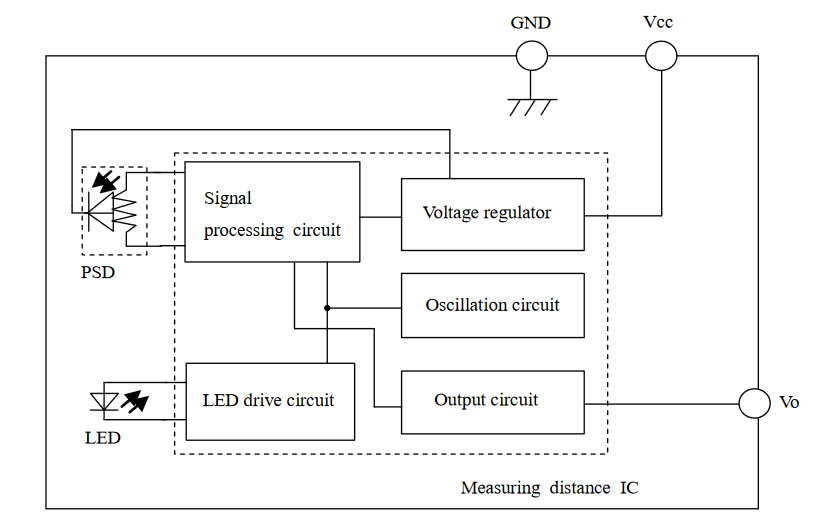
\includegraphics[width=0.8\textwidth]{figures/hardware/sensorData.PNG}
    \caption{Internal schematic of the distance sensors}
    \label{fig:sensorsData}
\end{figure}

\FloatBarrier

\noindent
Instead of connecting the voltage feed directly to 5V, we use a P-channel MOSFET to turn the sensors on and off at will. The connection of the transistor is the opposite of the N-channel described above (Section LEDs) and its functionality is the same: It is used as a switch. Notice the 47k resistors that connect the gates of the transistors to the pins of the mcu. By offering current from the pins, we close the switch and activate the sensors. Being able to turn the sensors on and off mostly offers flexibility in software.

Last, we feed the incoming data from the sensors to dedicated analog pins in our mcu.

\vspace{1cm}


\subsection{Components}

In this section, we list the actual components we chose to order. Most of the components were ordered from \textit{RSComponents}, Fig. \ref{fig:compRS} and the rest from \textit{Mouser}, Fig. \ref{fig:compMou}. The purpose of the lists provided are simply for reference. The components chosen are not a unique solution. Also, the choice of supplier was mostly made due to component availability reasons.

\begin{figure}[htb]
    \centering
    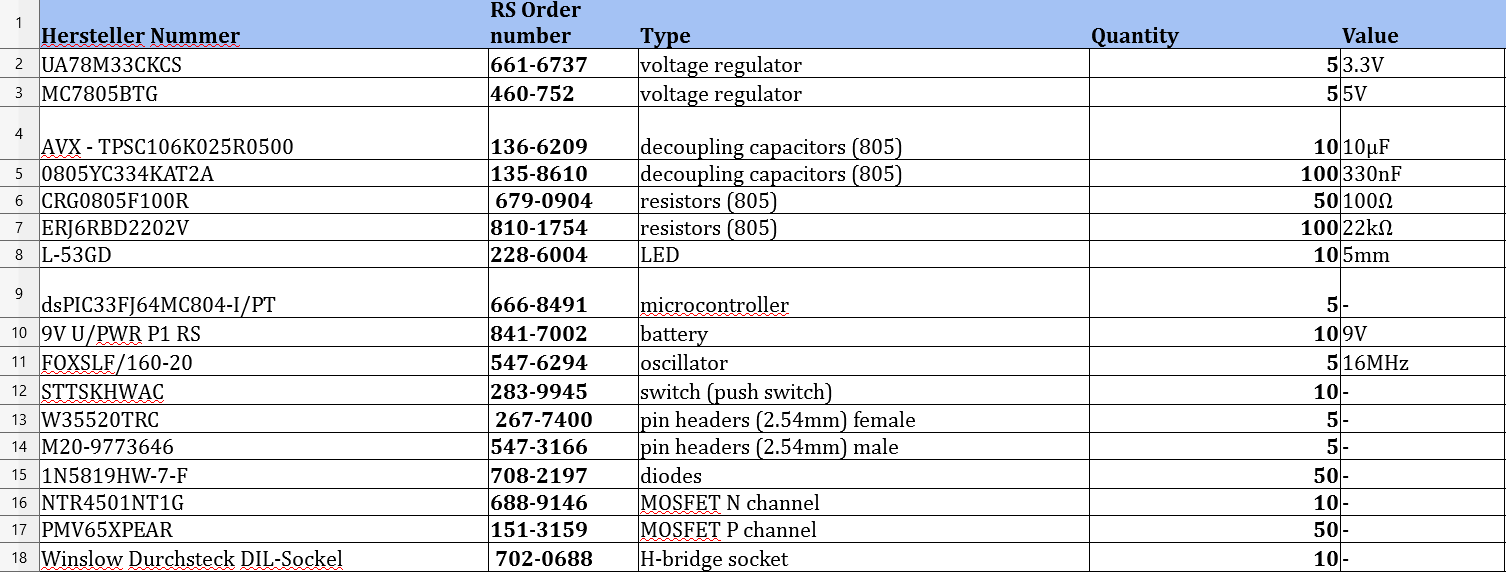
\includegraphics[width=1\textwidth]{figures/hardware/Components1.PNG}
    \caption{Components ordered from RSComponents}
    \label{fig:compRS}
\end{figure}


\begin{figure}[htb]
    \centering
    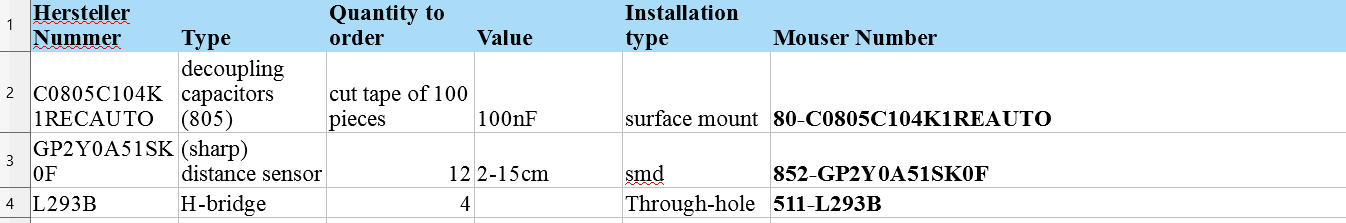
\includegraphics[width=1\textwidth]{figures/hardware/Components2.PNG}
    \caption{Components ordered from Mouser}
    \label{fig:compMou}
\end{figure}

\FloatBarrier
\noindent
Notice that the quantities mentioned are not referring to one board only. The quantities ordered were chosen with the thought of building four PCBs, checking the availability of existing components in the lab and the minimum components order of the suppliers. 
For the number of components needed per board, please refer to the Schematic and Fig. \ref{fig:comp1} and \ref{fig:comp2}.

\begin{figure}[htb]
    \centering
    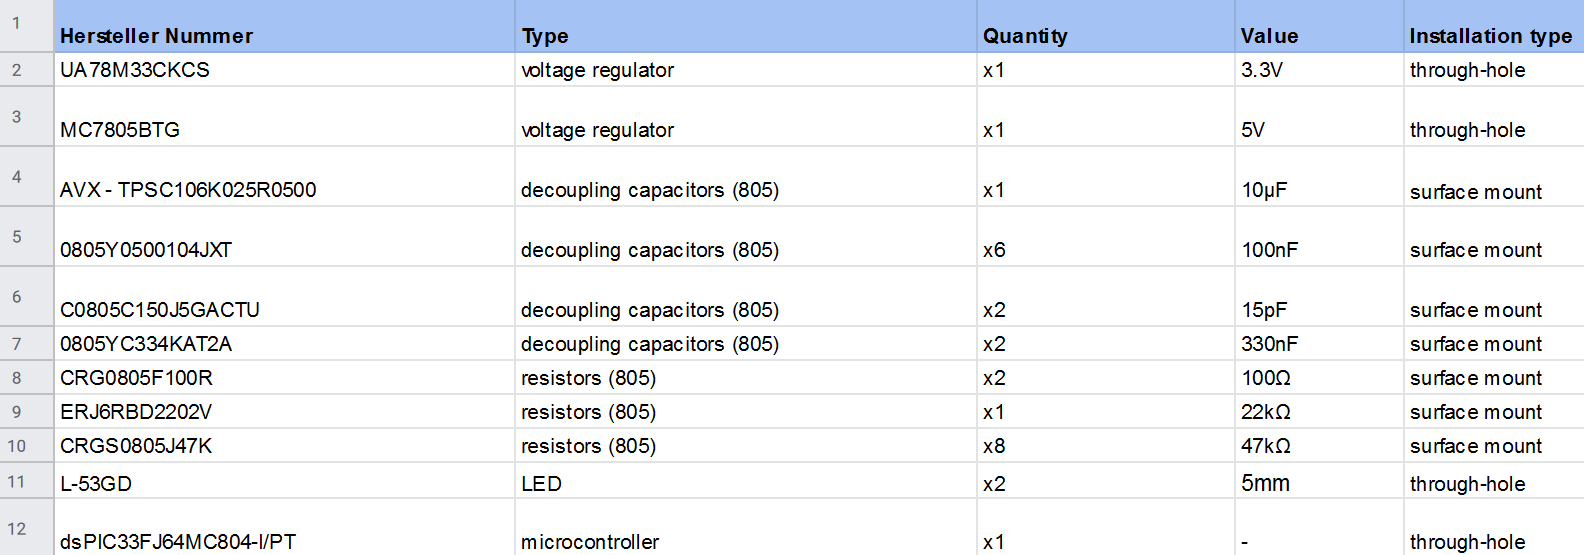
\includegraphics[width=1\textwidth]{figures/hardware/CompList.PNG}
    \caption{List of components needed for one PCB}
    \label{fig:comp1}
\end{figure}


\begin{figure}[htb]
    \centering
    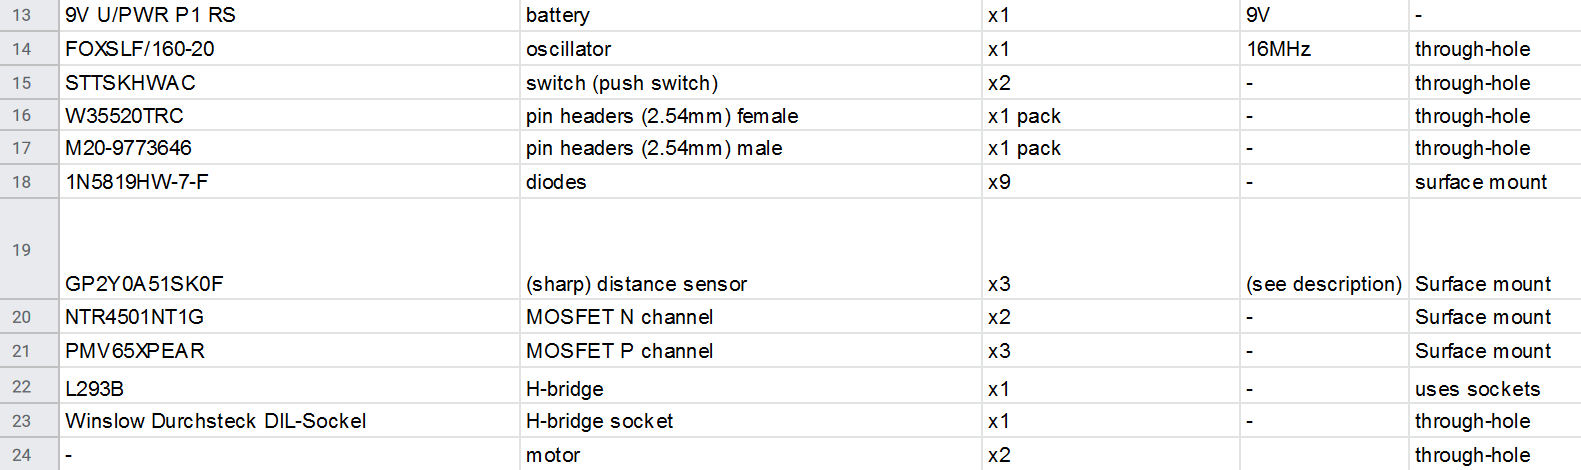
\includegraphics[width=1\textwidth]{figures/hardware/CompList2.PNG}
    \caption{List of components needed for one PCB (cont.)}
    \label{fig:comp2}
\end{figure}
\FloatBarrier

\vspace{1cm}


\subsection{Printed Circuit Board (PCB)}

In this Section, the PCB of the micromouse will be presented. All in all, the PCB is the body and soul of the robot: Its physical aspect constitutes the largest part of the robot, hosts the mcu (the brain of the robot) and all the necessary components already described in the Schematic Section. 
The finished PCB can be seen in Fig. \ref{fig:pcb}. The dimensions are: From head to tail 11.6 cm and from side to side 8.5 cm. The printed PCB can be seen in Fig. \ref{fig:print} .

\begin{figure}[H]
    \centering
    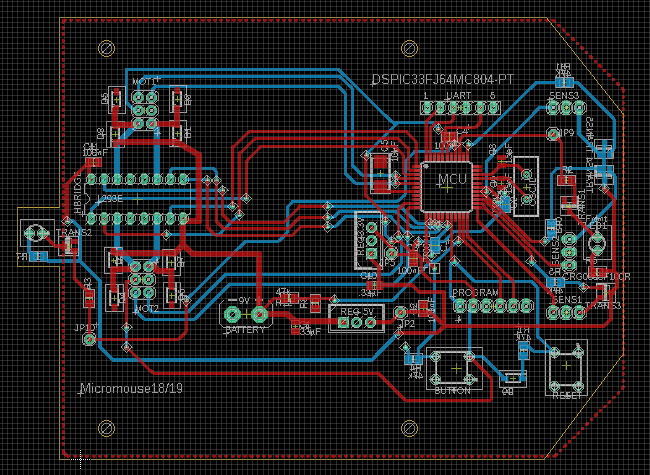
\includegraphics[width=0.8\textwidth]{figures/hardware/PCB.PNG}
    \caption{The final PCB version}
    \label{fig:pcb}
\end{figure}

\begin{figure}[H]
    \centering
    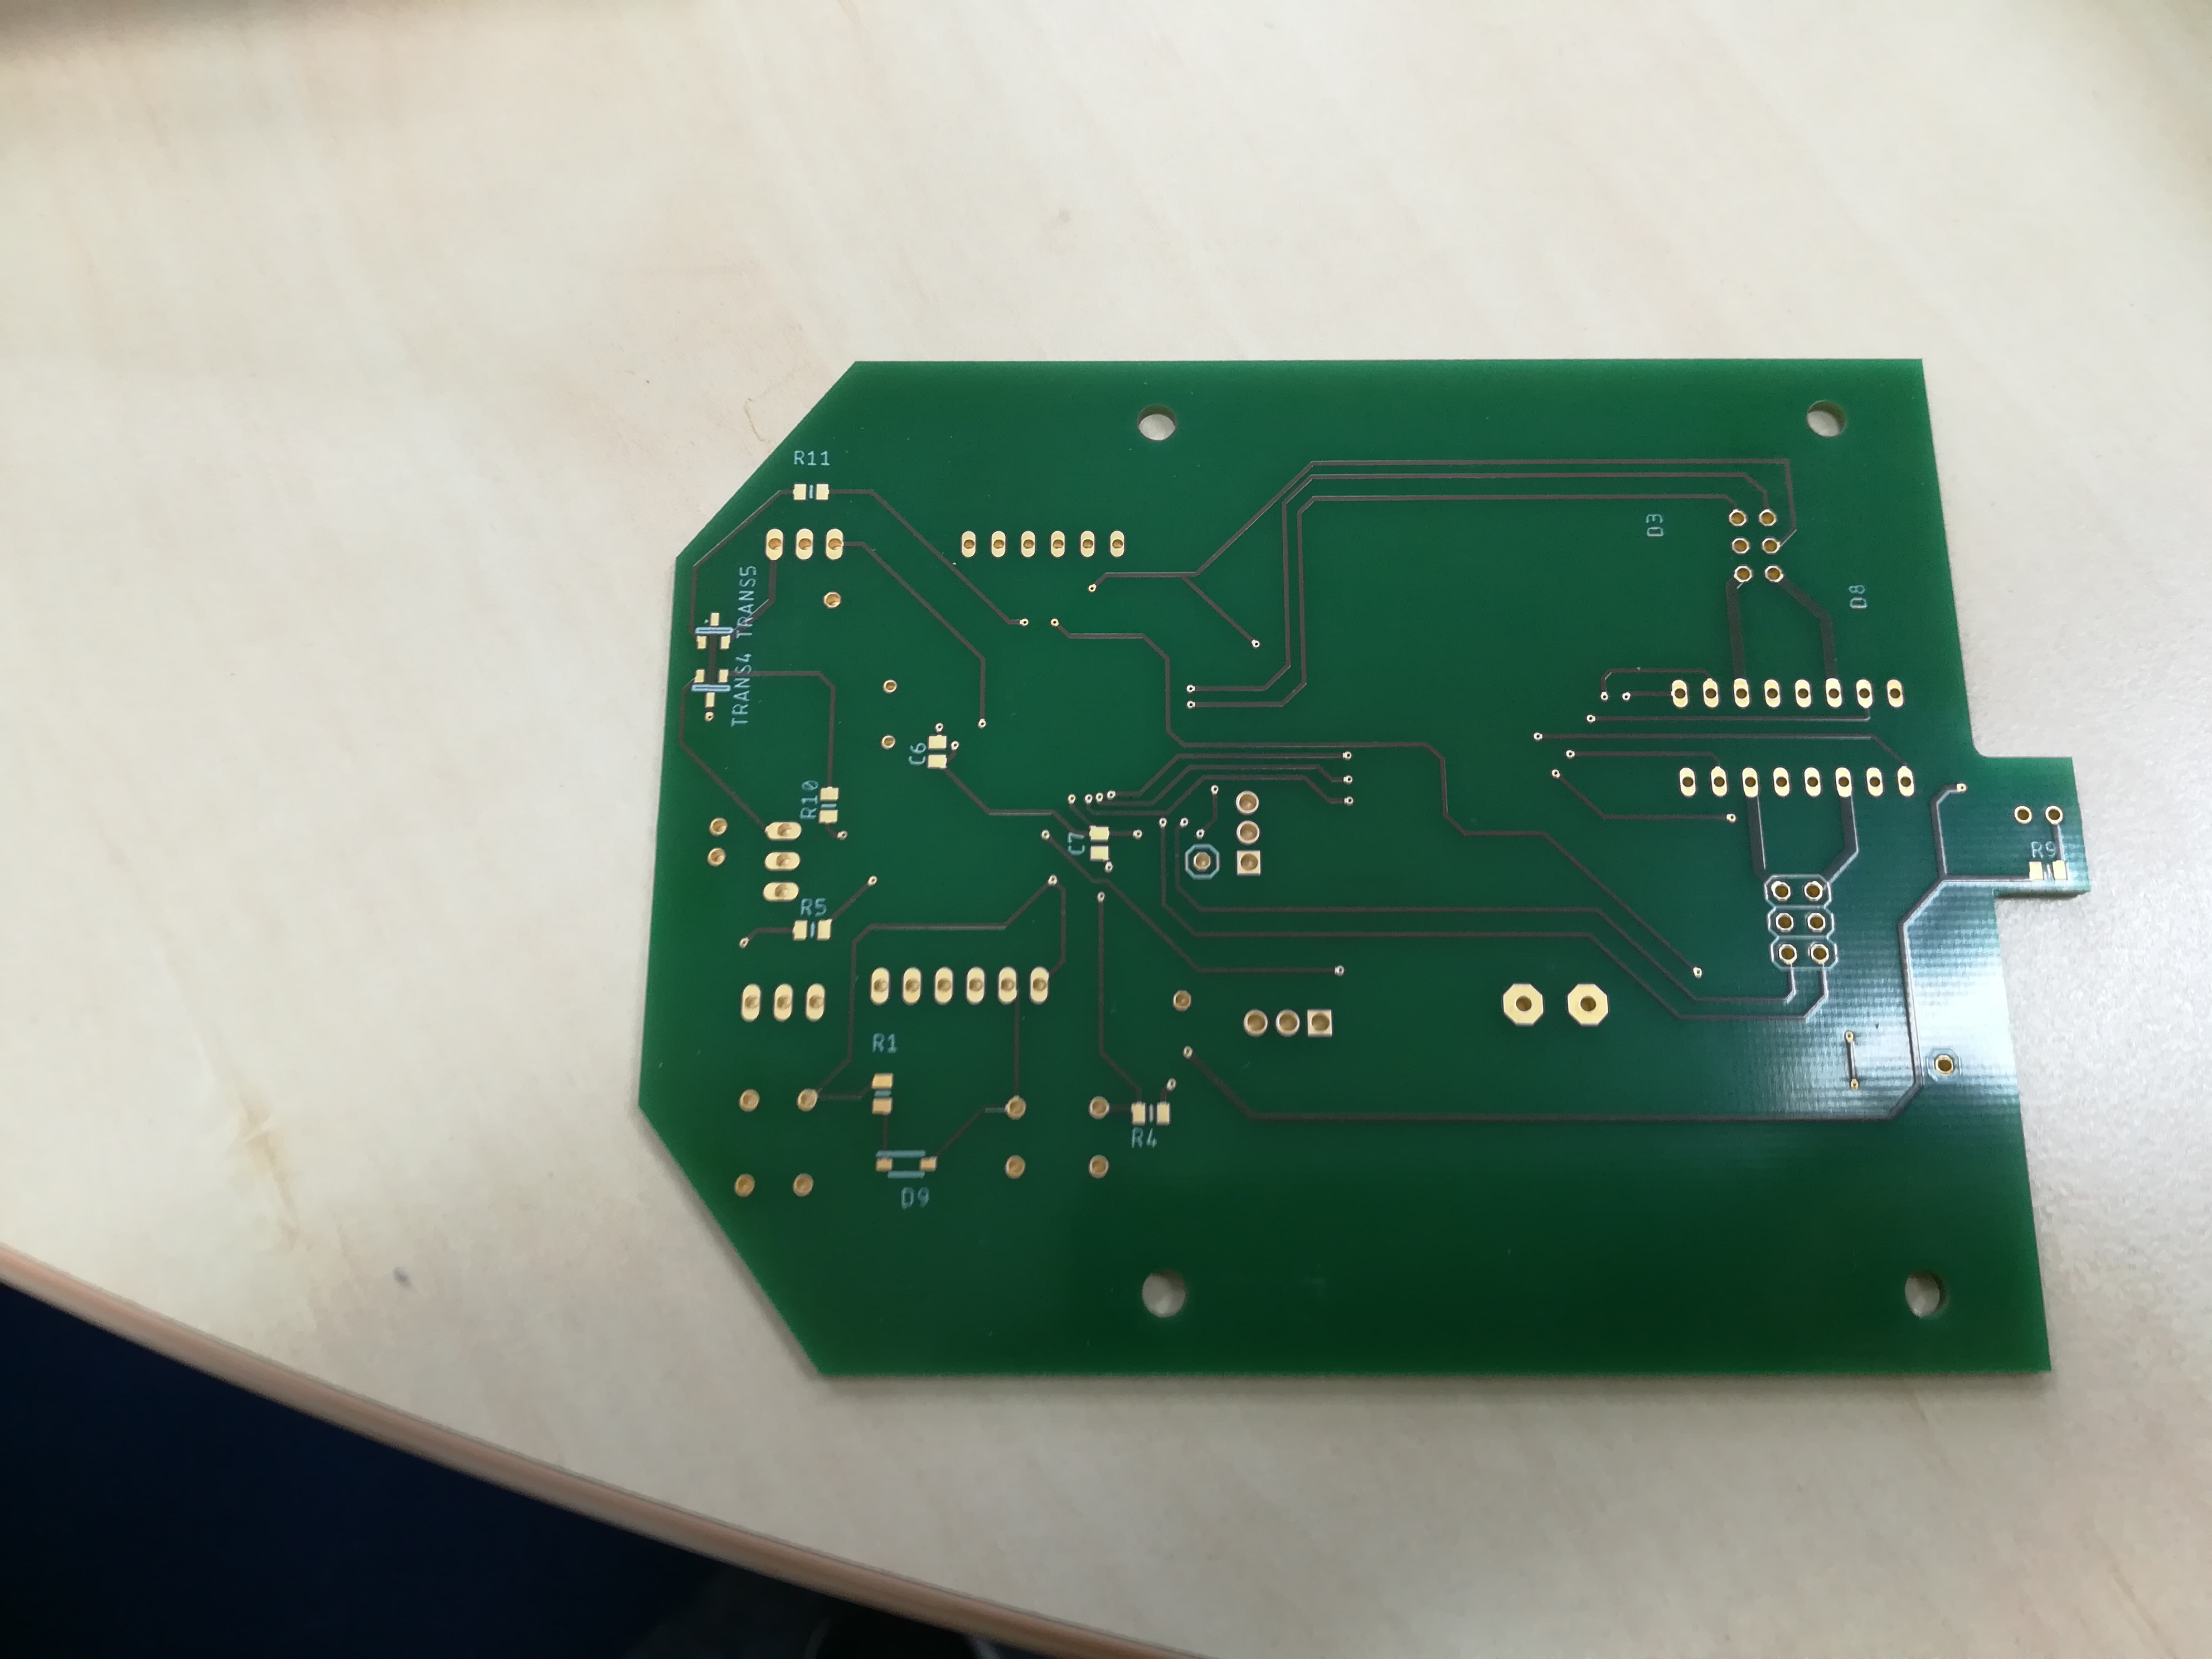
\includegraphics[width=0.8\textwidth]{figures/hardware/printed.jpg}
    \caption{The printed board (bottom layer)}
    \label{fig:print}
\end{figure}

\noindent
Our PCB features two layers: The top and bottom layer. Keep in mind that they are both physically and electrically isolated, unless we deliberately create a connection, as explained later. All necessary concepts are explained when needed in the following subsections, so it is important to read through them in order.\\
The process roughly consists of three steps, corresponding to the subsections that follow.

\FloatBarrier

\subsubsection{Components Placing}

Generating the PCB board from the Schematic is straight-forward in Eagle: The software offers an empty board and the models of the Schematic components placed out of it.

The first step of the procedure is to actually place the components on the board. There are no hard restrictions here, but rather a few rules of thumb. For example, it is desirable to reduce the size of the PCB as much as possible, but still place the components comfortably enough for connections to be made (traces). So a good trade-off has to be found. Before we continue with more examples of such rules, there are few details that need to be mentioned.

It is important to notice here, that the casing of the components was chosen as 805 and not smaller. We wanted a size that would allow us to comfortably solder the components on the board.

The final placement of components can be seen in Fig. \ref{fig:comp}.

\begin{figure}[htb]
    \centering
    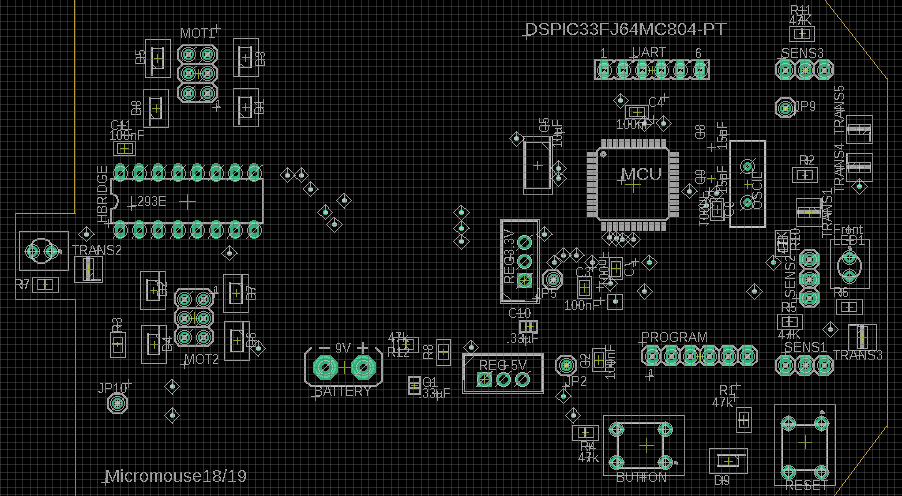
\includegraphics[width=0.8\textwidth]{figures/hardware/PCB_Components.PNG}
    \caption{The final placement of components on the PCB}
    \label{fig:comp}
\end{figure}

\noindent
As mentioned, in our case, a two layer PCB is designed. The top and bottom layers, both contain components. To fully appreciate this fact, notice that there are two different kinds of components used on a PCB: Through-hole and surface mount (SMD). 

The through-hole components actually go through the PCB. The manufacturer needs to drill holes for this purpose. An advantage of this type is mechanical stability. Another advantage comes in the tracing phase, when connecting the components: The through-hole ones can have traces leading to and from them in both the top and bottom layers. The reason is obvious, they have physical presence in both layers, since they go through the surface of the PCB to the other side. However, the whole concept does occupy more space than the SMD components. Also, drilling holes costs more, when ordering the PCB.

Now the SMD components are soldered only on the surface of the PCB (top or bottom layer) and no drilling is required. They occupy less space too. However, a track can lead to or from them only in the layer they are found. If a connection between SMD components in different layers needs to be made, a change of layer on the track is necessary, somewhere in its course. We will come back to tracing in the next subsection. 

\FloatBarrier
\vspace{1cm}

\noindent
For now, let us consider some of the needs that led to this particular placement of components. The following train of thought is definitely not unique and a different placement could have been chosen.

Referring to Fig. \ref{fig:comp}, let's start with the sensors' pin headers. It is clear that the distance sensors need to  be placed in the front (right side of the PCB). Therefore their pins have to be placed nearby. Now, notice the analog nature of the sensors output: We want the traces of those signals to the mcu to be as short as possible, since analog signals are susceptible to noise. Hence the mcu is placed in the front of the board, as well.

After this choice is done, the location of several components is obvious: The oscillator needs to be as close as possible as well. The decoupling capacitors, whether on the top or bottom layer, need to be placed as close to their connecting pins, as possible. It is a good idea to also place the programmer and the UART pin headers close to the mcu for convenience.

The buttons need not necessarily be placed close to  the mcu. Admittedly, a more convenient location for them could be found on the board, for example one in the front and one in the back.

Notice the empty space in the middle of the board. It is planned for the battery. In our case, instead of using a through-hole battery case on the board, the battery is to be floating above it, in a dedicated case of the casing. Even though it would be possible to dismiss the space kept on the board, we chose to keep it as a plan B, just in case the casing is not available. To the left and right of the battery more space is kept for the motors, dictated by their dimensions and the casing to host them. Finally, notice the four drills at the left and right sides of the board. As will be explained later, the design of the casing allows for sliding the board in it, before the motors and wheels are placed. However, just in case extra stability is needed, these four holes allow for screws to hold the PCB and the casing together.

Since we are still in the middle of the board, notice the two voltage regulators, in succession of the battery pins. It is convenient, in our case, to have the source in the middle of the board.

Moving on to the back of the PCB, the H-bridge needs to be placed in the middle of the two motors' pins. The back LED, much like the front one in placed approximately in the middle of the edge, since its role is mechanical stability. The little tail, where the LED is placed, is just a nice artistic touch, as are the front cuts on the board.


\subsubsection{Tracing (Connecting Components)}

Now that the components have been placed and the shape of the PCB decided, they need to be connected. This procedure is called "tracing", since the components are connected through copper traces on the board.
As mentioned above, the traces can be on the top or bottom layer and the two layers are isolated, hence the traces on different layers are also isolated from each other. 
The final tracing can be seen in Fig. \ref{fig:pcb} above.
A view with the traces on the top layer can be seen in Fig. \ref{fig:top}. The view featuring only the traces on the bottom layer can be seen in Fig. \ref{fig:bottom}.

\begin{figure}[htb]
    \centering
    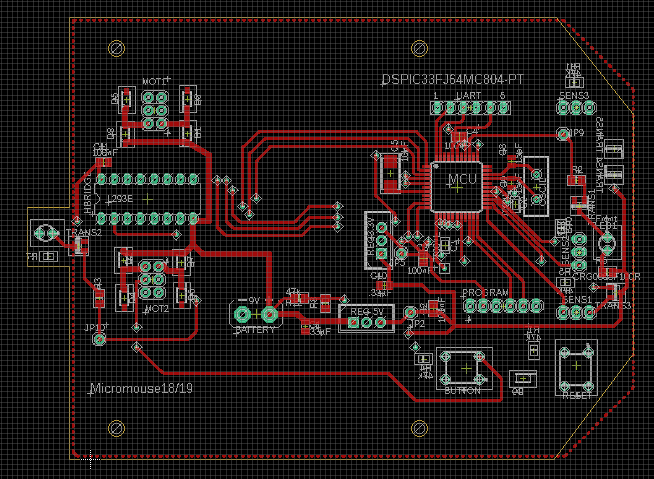
\includegraphics[width=0.8\textwidth]{figures/hardware/PCB_Top.PNG}
    \caption{The PCB with only top layer traces visible}
    \label{fig:top}
\end{figure}

\begin{figure}[htb]
    \centering
    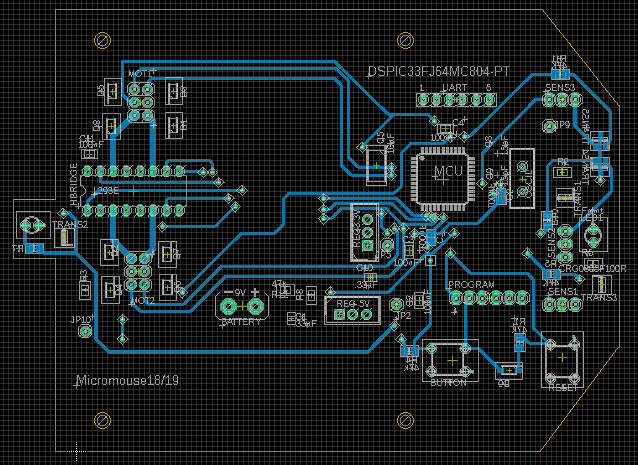
\includegraphics[width=0.8\textwidth]{figures/hardware/PCB_Bottom.PNG}
    \caption{The PCB with only bottom layer traces visible}
    \label{fig:bottom}
\end{figure}

\FloatBarrier
\noindent
This is a good point to introduce the concept of "via points". Notice how traces on the top layer (red) change to traces on the bottom layer (blue) and vice versa. The point where the layer (and color) changes is a via point. A via point is a drill on the PCB, to allow for the trace to change layer. 
Hopefully, the above discussion about SMD and through-hole components makes more sense now. Notice how, in some cases, the traces change layer just before connecting to an SMD component, in order to get to the component's layer.
All in all, drawing traces in an organized manner is not straight-forward. Two restrictions to keep in mind: Keep both the number of via points and the length of the traces as low as possible. The reason for the first being the cost and complexity of the PCB and for the latter, the cost and the accuracy of the corresponding signal: The longer the trace, the larger its resistance, the bigger the noise that is picked up.

One important aspect of tracing is the choice of trace width. So to speak, professionals quickly develop a feeling for this, but for the rest of us, there is always the scientific way:

The total resistance of a trace is given by the following formula

$$R = \rho * \frac{l}{A}$$

\noindent
Here, $\rho$ is the specific electrical resistance of copper (as material). It equals to $1.68*10^{-8} \Omega *m$ at $20 \degree C$.
l is the length of the trace and A is the height of the trace (usually 0.035mm) multiplied with the width.
In order for the right width to be chosen, we need to consider the desirable value for the resistance. And in order to do that, again $\Omega$hm's Law has to be considered, referring to the current we expect to run through our trace.
This analysis leads to the intuitive result: When we expect a large value for the current, then a smaller resistance is needed and thus a larger width value for the trace needs to be selected. For smaller values of current, smaller width may be selected. In any case, a minimum width is dictated by the manufacturer rules and the good connection of a component's pin.

For example, it is known that motors can draw a lot of current, especially when they first start moving. Thus, the traces to the motors and the H-Bridge need to have a wider width.

Eagle offers a nice feature when it comes to measuring trace length and acquiring an estimation of relevant values. A ULP script provides us with this info, by running the command \textit{run length-freq-ri} in Eagle's command line. An example from our circuit can be seen in Fig. \ref{fig:length}. Notice how the estimation for the maximum current on the trace is shown in the end right column and how the wider traces of the motor (e.g. M1+, M2+, etc.) can take more than 1A.

\begin{figure}[H]
    \centering
    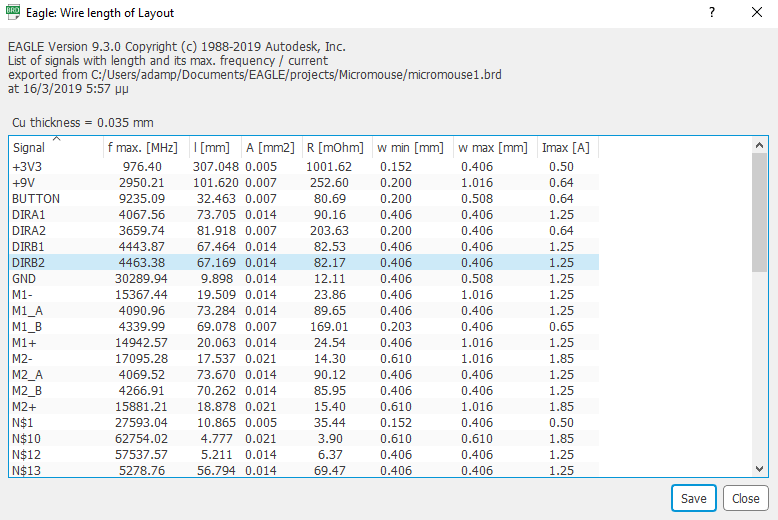
\includegraphics[width=1\textwidth]{figures/hardware/ULP.PNG}
    \caption{Trace length and other info}
    \label{fig:length}
\end{figure}

\noindent
All in all, we kept it simple and well in the limits with  the choice of the width: There are only three different widths in our PCB traces. The largest is 1.016 mm and is used for the connections between the motors, the H-bridge and the battery. Then we have 0.6096 mm for the connections from the 5V regulator (essentially the sensors). Last, the smaller width is 0.4064 mm and is used for all the rest. Especially in the case of the close to each other mcu pins, a larger width would be a nuisance, since there needs to be a minimum clearance between the traces.

\vspace{1cm}

\noindent
The last concept to be introduced in this chapter is the "ground plane" (GND). The ground plane is a convenient way of connecting all the GND nodes (pins) of the components, meaning the pins that need to be connected to 0V. For our purposes here, we will call it ground. In essence, it is a layer that can be placed on a PCB layer, which connects everything on it. It can be seen in Fig. \ref{fig:gnd}.
In reality, there is a much more important motivation to create a GND plane, instead of connecting pins of components like with positive voltage: Noise rejection. We will not go into this here, but it is worth considering the noise signals coming out of the pcb and the ones produced from the pcb. Closed traces of high-frequency current may function as antennas, when the space they encompass is large. This would be the case if one used traces also for the 0V connections. By using a GND plane, however, this area is kept to a minimum, limiting the noise produced.

\begin{figure}[htb]
    \centering
    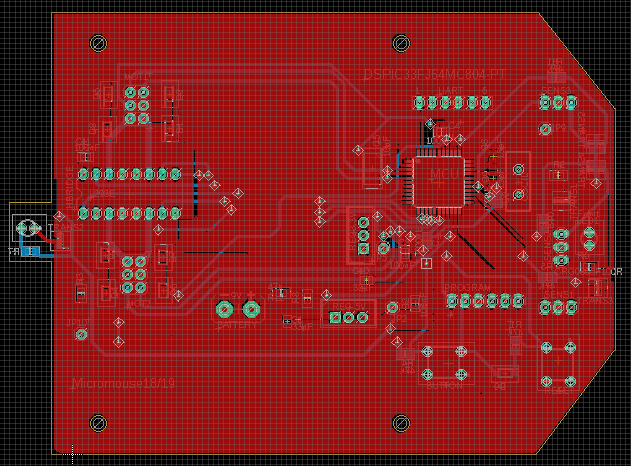
\includegraphics[width=0.8\textwidth]{figures/hardware/PCB_Grounded.PNG}
    \caption{The PCB with the ground plane visible}
    \label{fig:gnd}
\end{figure}

\noindent
The copper traces run through this all-connecting surface, in order to connect the necessary pins. This is especially visible in the above pictures of the actual PCB, where the green entire surface is GND and the tracks running through it are the traces mentioned above, playing the role of wires in a physical circuit.

The GND surface can be applied to one of the layers or both. In our case, we placed one only on the top layer,since the SMD components on the bottom layer that needed to be connected to GND were very few. The solution might not seem very elegant, but is functional: A trace runs from the gnd pin of the component, on the bottom layer, and ends in a via point. Hence, it connects to the GND on the top layer. An example from our circuit can be seen in Fig. \ref{fig:via}.

\begin{figure}[htb]
    \centering
    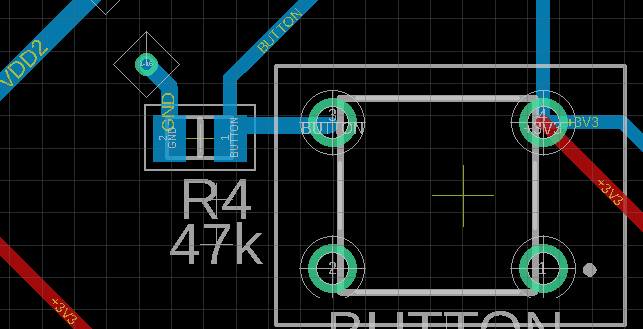
\includegraphics[width=0.8\textwidth]{figures/hardware/Via.PNG}
    \caption{How an SMD component on the bottom layer connects to the GND surface on the top layer}
    \label{fig:via}
\end{figure}

\FloatBarrier

\subsubsection{Design Rules Check (DRC)}

Once the traces are in place, a final check has to be performed, before the board is handed to the manufacturer. Luckily, Eagle provides a straight-forward tool to check for minimal distances between components and traces, overlapping, floating connections and other issues: The DRC (Design Rules Check).

In our case, the manufacturer PCB-Pool provides a set of their own rules about minimum trace width, via points, clearance rules etc. After incorporating it in Eagle and checking, all of the found issues need to be fixed, before the board is ready for production.
An instance of the interface can be seen in Fig. \ref{fig:drc}.

\begin{figure}[htb]
    \centering
    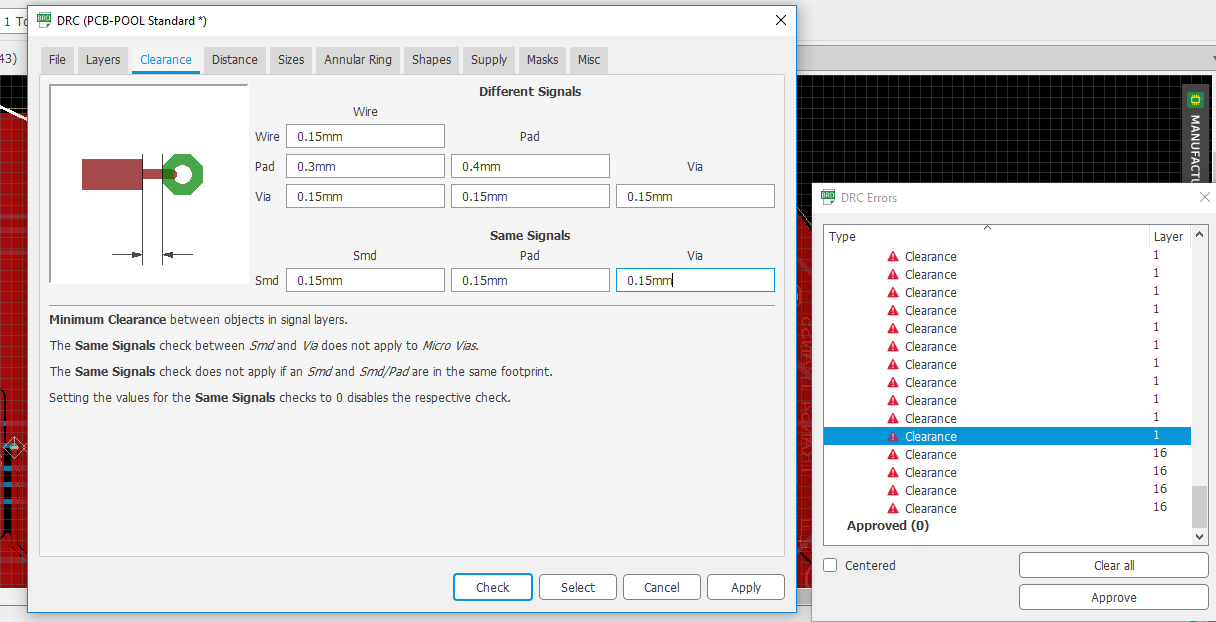
\includegraphics[width=1\textwidth]{figures/hardware/DRC.PNG}
    \caption{Interface of DRC and list of found violations}
    \label{fig:drc}
\end{figure}


\FloatBarrier
\vspace{1cm}

\subsection{Casing}

To house not only the PCB, but also sensors ,motors and the battery in a safe and robust way, a set of casing for the micromouse is designed and 3D printed.

\begin{figure}[htb]
    \centering
    \begin{minipage}{.45\textwidth}
          \centering
            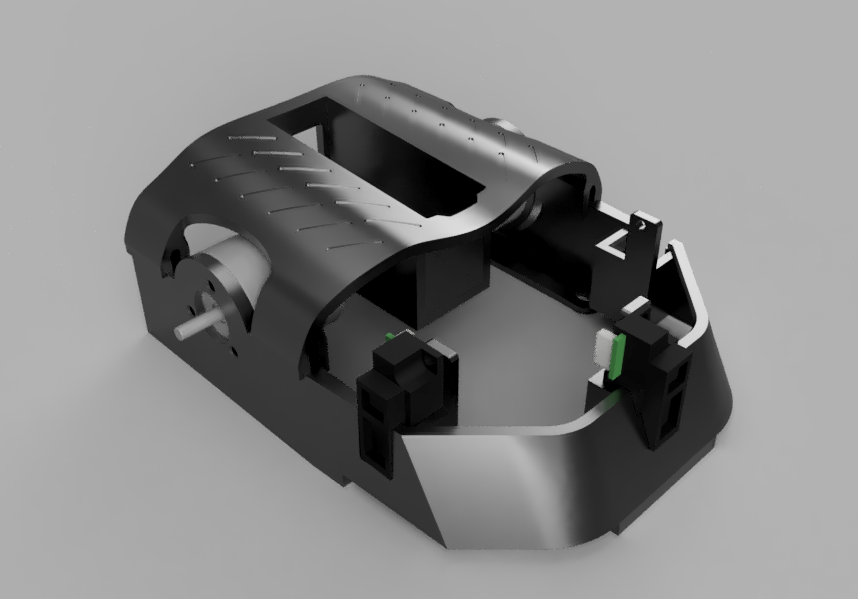
\includegraphics[width=.9\linewidth]{figures/Casing/CADrendering.png}
              \caption{A rendering of the MicroMouse casing CAD 3D Model}
    \end{minipage}
    \begin{minipage}{.45\textwidth}
          \centering
            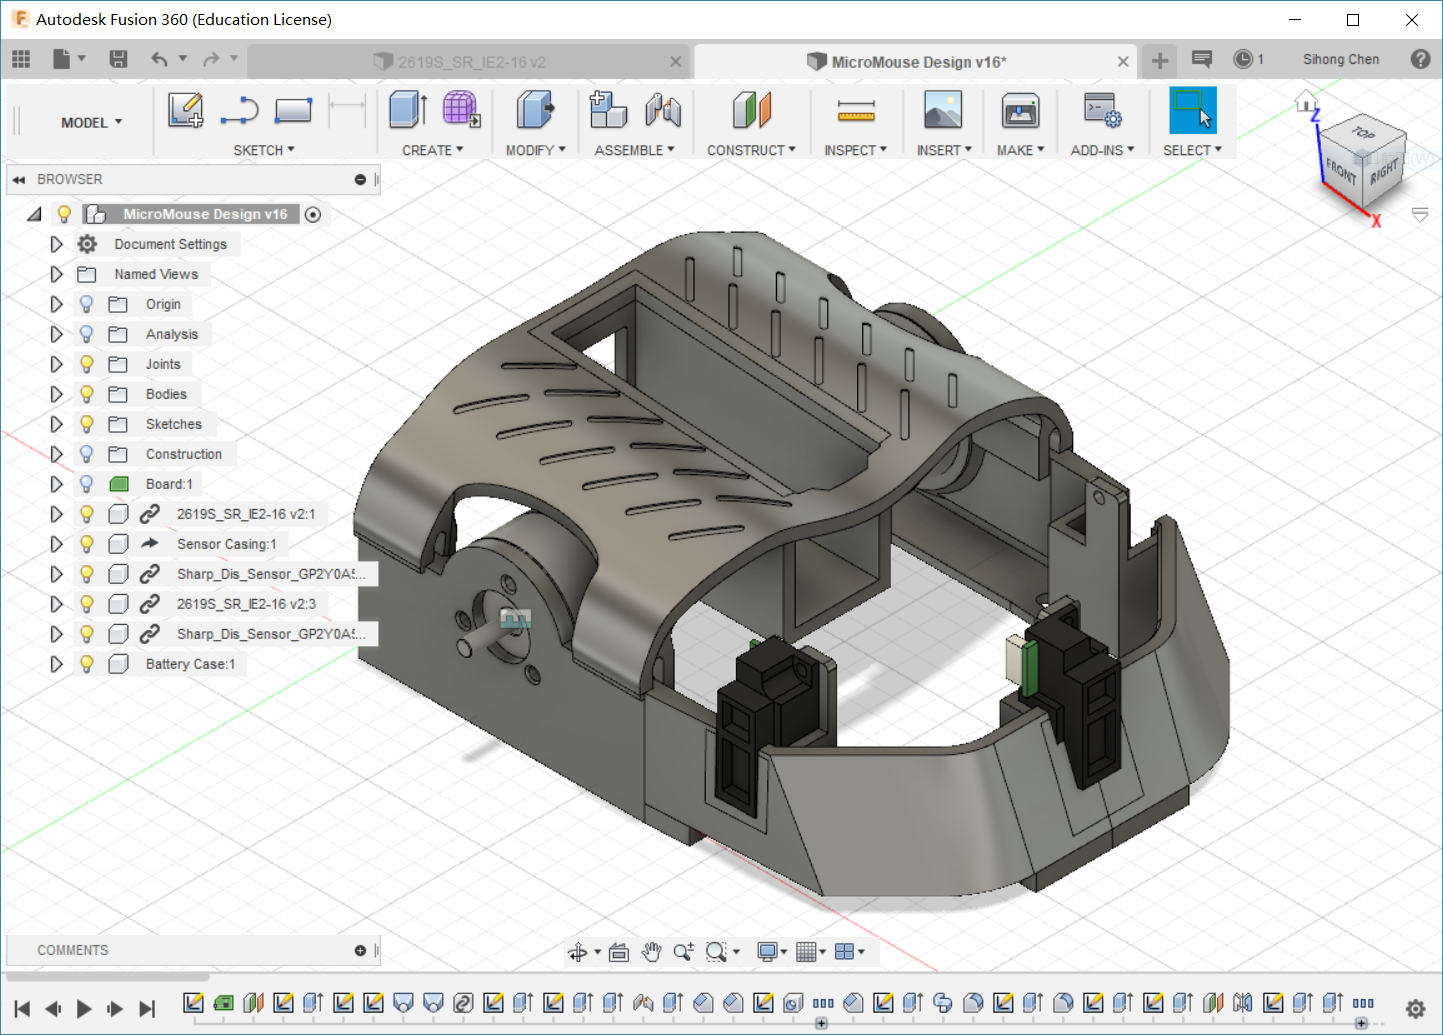
\includegraphics[width=.9\linewidth]{figures/Casing/FusionModelling.PNG}
              \caption{MicroMouse casing in Fusion 360 CAD modelling environment}
                \label{fig:CaseModelling}
    \end{minipage}
\end{figure}

\subsubsection{CAD Modelling}
\begin{itemize}
    \item Base Casing\\ 
    This casing is the encompassing platform, on which all hardware components are placed. See figure \ref{fig:CaseModelling} for the CAD model of the base casing.

    PCB rests on the bottom wrapper, and is fastened on with screws. Motors are mounted on the side with screws as well. Sensors are placed one front centre, another two facing left and right.

    In this CAD model, there are several components. Other than the base wall, the most prominent components are the sensor casings. These are actually one component, but imported on three positions, modified according to other components and integrated into the assembly design. 

    The approach to model the sensor casing separately as a component and later integrate reduces duplicate work. This separation also ensures that even a change in sensor model would only result in limited modification work to the final design.
    

    \item Battery Cover\\ 
    In order to secure the battery safely and make our robot space efficient, a battery cover is designed to hold the battery above PCB and other components. It also serves as a covering case for aesthetic purposes to some extent.

    This cover is designed to be a snap fit with the base casing, see figure \ref{fig:SnapFitBase} and \ref{fig:SnapFitCover}.

    For designing the surface of this cover, the free-form modelling and sculpting feature is used, in addition to the more traditional parametric modelling and solid modelling. This allows us to more easily model a visually pleasing surface to the design, giving our mouse a more “sporty” look, rather than the usual “boxy” appearance from more traditional CAD methods.

    In the design of the battery cover, attention was paid to reduce overhanging structure, so that the supporting structures needed are minimised. For example, the front side of the battery holder is left empty, as it eliminates support structure when this part is printed vertically (front is facing up). However, some support is unavoidable, for example when there is enclosing structure such as a circle.

\end{itemize}

\begin{figure}[htb]
    \centering
    \begin{minipage}{.45\textwidth}
          \centering
            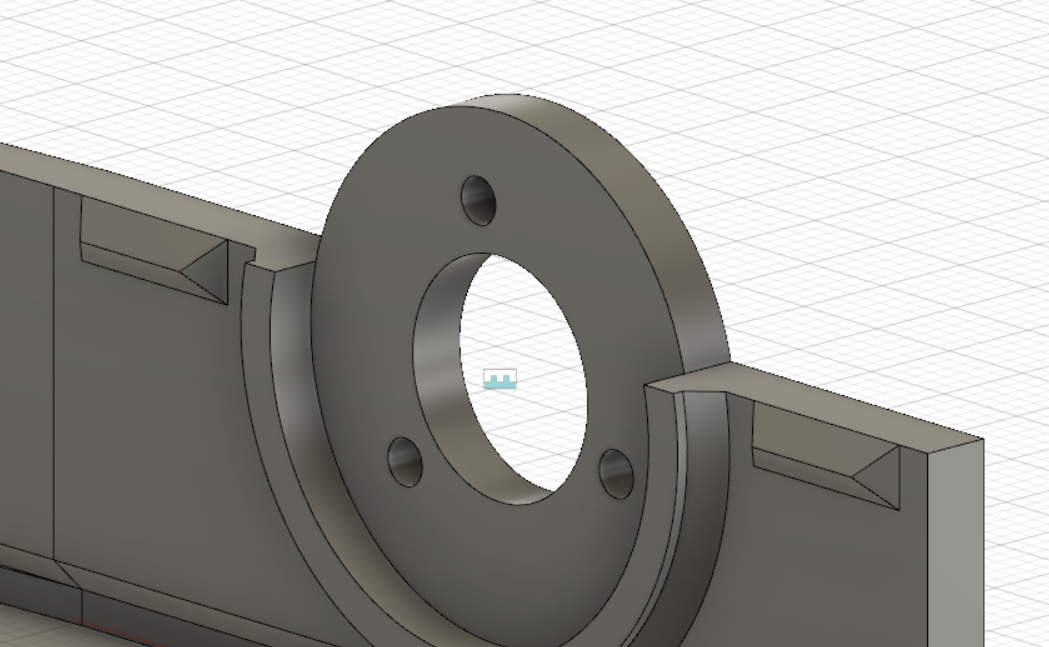
\includegraphics[width=.9\linewidth]{figures/Casing/SnapFitBase.PNG}
              \caption{Snap fit design on the base part}
                \label{fig:SnapFitBase}
    \end{minipage}
    \begin{minipage}{.45\textwidth}
          \centering
            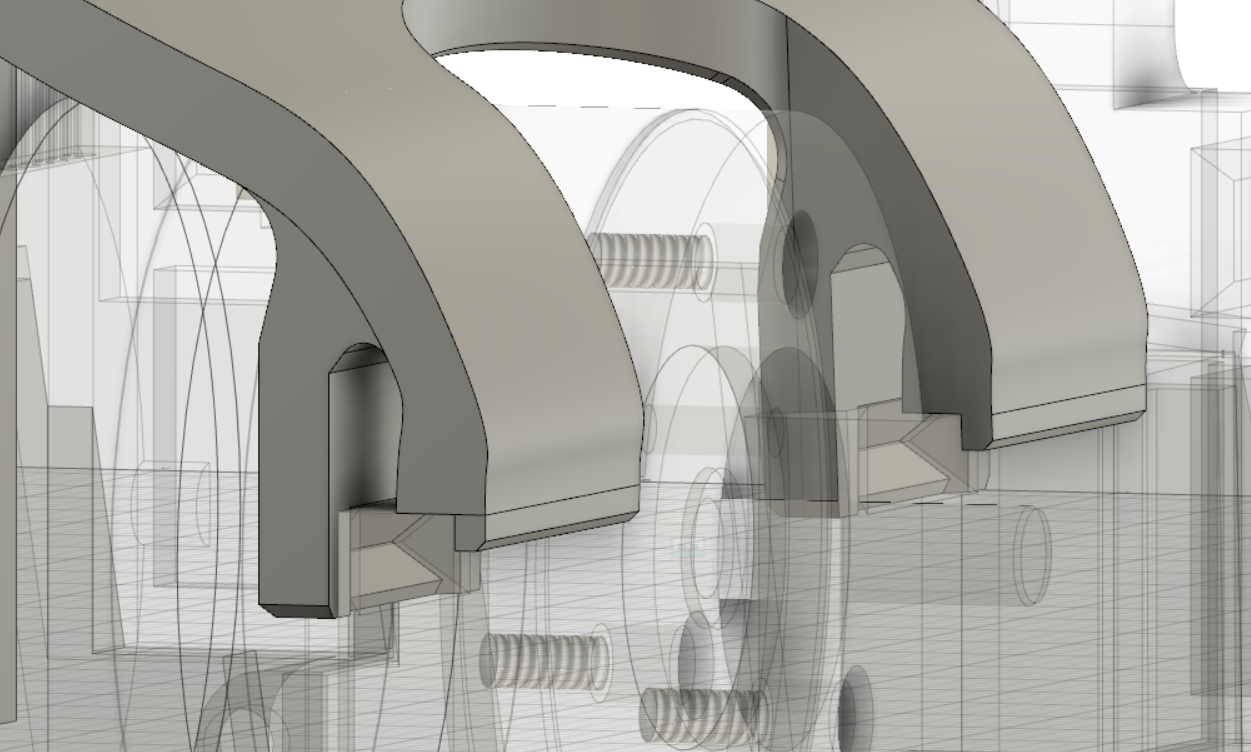
\includegraphics[width=.9\linewidth]{figures/Casing/SnapFitCover.PNG}
              \caption{Snap fit design on the cover part}
                \label{fig:SnapFitCover}
    \end{minipage}
\end{figure}

\subsubsection{3D printing the casing}
\begin{itemize}
    \item Method\\ 
    There are many types of 3D printing process, most common ones include Material Extrusion method such as Fused Deposition Modeling (FDM), and Vat Polymerization such as Stereolithography (SLA), Direct Light Processing (DLP). FDM is most widely available method of 3D printing, meanwhile SLA has a better dimensional accuracy (lower limit $\pm$ 0.10 mm in a desktop SLA printer compared to lower limit $\pm$ 0.5 mm in a desktop FDM printer).

    The 3D printing method we used is Fused Deposition Modeling (FDM). Out of the two available 3D printer FDM and SLA, the FDM method is chosen for its shorter lead and print time, as it does not require a curing process as for SLA. The dimensional accuracy is also acceptable to our application.
    
\begin{figure}[htb]
    \centering
    \begin{minipage}{.45\textwidth}
          \centering
            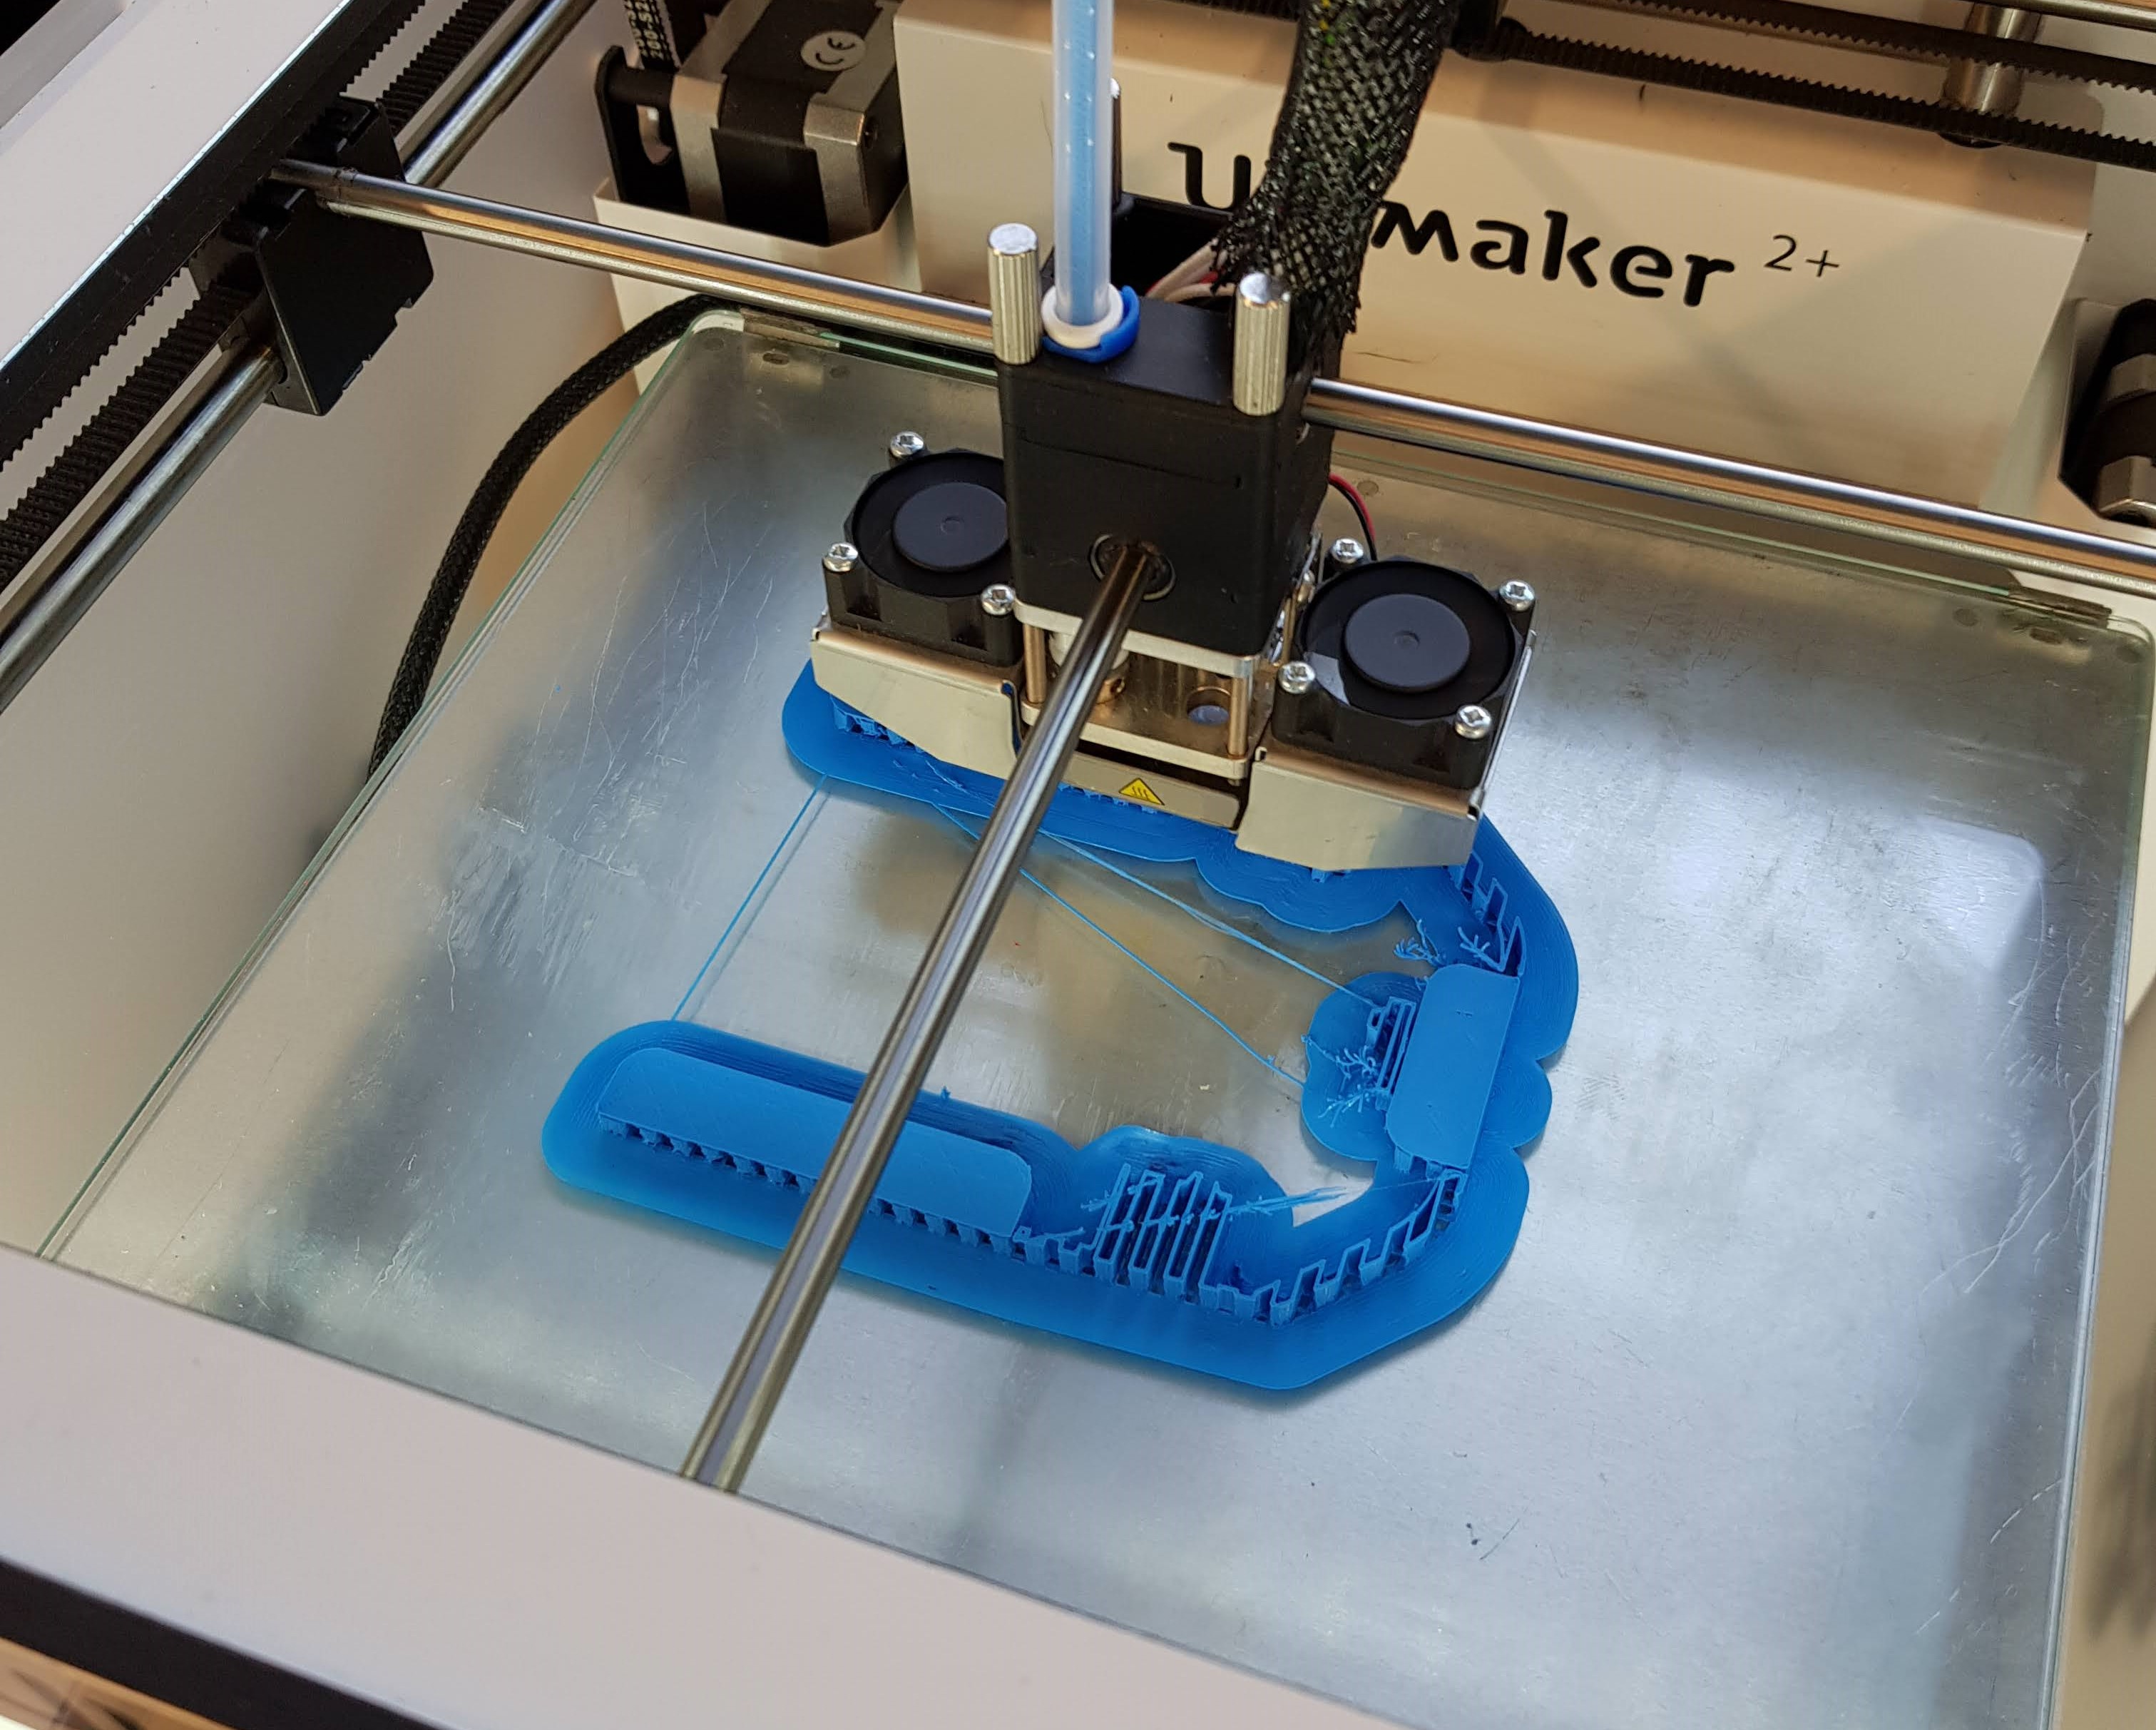
\includegraphics[width=.9\linewidth]{figures/Casing/PrintingProcess.jpg}
              \caption{A Case being printed}
    \end{minipage}
    \begin{minipage}{.45\textwidth}
          \centering
            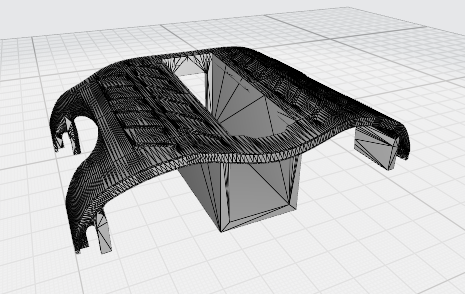
\includegraphics[width=.9\linewidth]{figures/Casing/Battery_Case_Micromouse_STL.png}
              \caption{Model in STL format for slicer program to process}
    \end{minipage}
\end{figure}
    
    \item Material\\ 
    There are two kinds of material for the FDM printer available for us, which are also the two most widely used materials for FDM 3D printing, namely PLA (Polylactic Acid) and ABS (Acrylonitrile Butadiene Styrene). They both can be used to print dimensional accurate parts, with very similar cost. PLA is under correct condition biodegradable, whereas ABS is not but recyclable.

    ABS is chosen for our project due to its improved ductility, higher flexural strength, and slightly better mechanical properties. Because ABS is less brittle than PLA, it has also better machinability, that means drilling hole or sanding would be easier, which we will likely do, whereas PLA would require more care during such post-processing.

    \item Process\\ 
    For this project, the 3D print process includes generating STL file from 3D CAD model, slicing and adding support structure, printing, and post processing work.

    One problem that often occurs during 3D printing is handling critical surface, therefore attention is paid to ensure that the critical surfaces in our design such as inside surface of sensor casing are all parallel or vertical to the platform plane, so that the 3D printer can produce a more precise and smooth result.

    Specialised programs or Slicers "cut" CAD models into layers and compute how the printer's extruder would assemble each layer. When necessary, support structures are also added in this stage, depending on if there is overhanging structures in the model.

    Post processing is mostly removing support structures from the printed parts, and sanding and polishing rough edges and surfaces.
\end{itemize}

\FloatBarrier
\vspace{1cm}


\section{Software design}
\textcolor{red}{some general info}

\subsection{Peripherals} %please think about the appropriate name!
The description of our modular architecture, the work principles of the separate modules and basically "how we control the peripherals" such as motors, leds, timers, etc. Logic comes a bit later in here.
Also all info on DMA and pin remapping and our pretty mapping table are also welcomed here I think

\subsubsection*{Timer 1}
\textcolor{red}{
Short description on how we worked out the time
}

\subsubsection*{Pulse Width Modulation (PWM)}

\begin{figure}[htb]
    \centering
    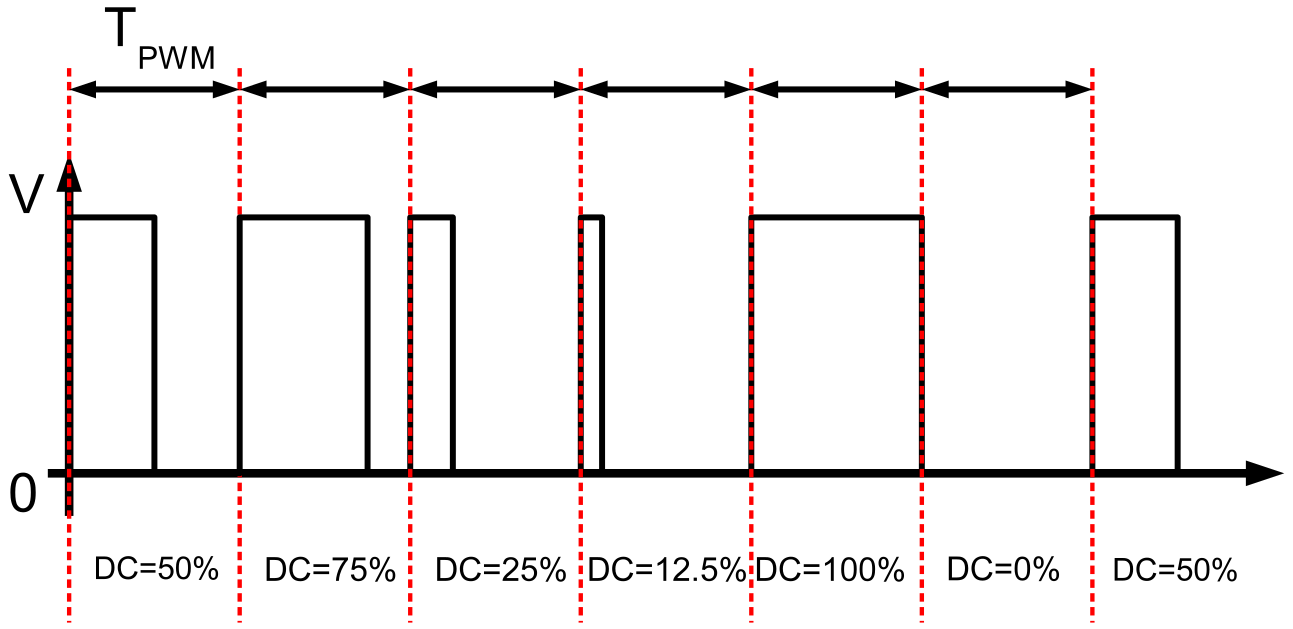
\includegraphics[width=0.6\textwidth]{figures/software/pwm_demo.png}
    \caption {Principle of PWM \cite{alex}}
    \label{fig:pwm_demo}
\end{figure}

Pulse Width Modulation allows us to control the amount of energy supplied to an actuator. In this case we use the PWM signal to drive our motors and control their speed. Using different pulse widths, we can supply different amount of power to our motors. \cite{alex}


As seen in figure \ref{fig:pwm_demo}, we have a fixed PWM period $T_{PWM}$. We can now vary the so called duty cycle $DC$ by changing the time the PWM output is switched on ($T_{DC}$).
\begin{equation}
    DC = \frac{T_{DC}}{T_{PWM}}
\end{equation}
For our PWM unit, we mainly have to choose the parameters:
\begin{enumerate}
    \item PWM period
    \item PWM duty cycle
\end{enumerate}


Depending on our PWM period, we get different amount of ripple in our resulting signal. More on this can be found in \cite[Chapter~5.1]{alex}. In figure \ref{fig:pwm_choice} is an example of possible choices for the PWM period register ($PTPER$) and the PWM duty cycle register ($PDC$)

\begin{figure}[htb]
    \centering
    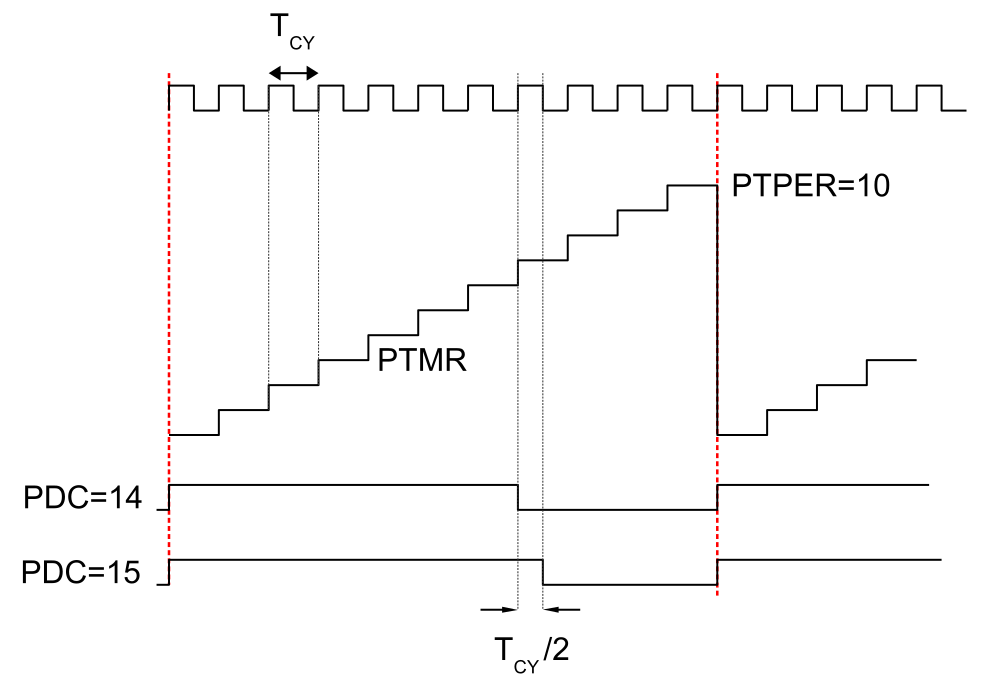
\includegraphics[width=0.6\textwidth]{figures/software/pwm_choice.png}
    \caption {Example: Resolution of PWM duty cycle \cite{alex}}
    \label{fig:pwm_choice}
\end{figure}

For our motors, we have the following parameters:
\begin{itemize}
    \item \textbf{fixed}: $T_{CY} = 25 ns$
    \item timer prescaler $PTCKPS = 0b00$ (option 1:1)
    \item PWM period register $P1TPER = 2000 - 1$
    \item PWM duty cycle $PDC \in [0, 2*(P1TPER + 1)]$
\end{itemize}
$T_{PWM} = ( PTPER + 1 ) * T_{CY} = 2000 * 25ns = 50000 ns$


$f_{PWM} = \frac{1}{T_{PWM}} = 0.25 * 10^{5} Hz$

With the current values, we can now set different duty cycles for our motors by choosing valid values for the $PDC$ register.


\subsubsection*{Quadrature Encoder Inferface(QEI)}
To measure the position and velocity of our motors, we are provided with a \textit{quadrature encoder}. The principle of a quadrature encoder is depicted in figure \ref{fig:qei_demo}. 

\begin{figure}[htb]
    \centering
    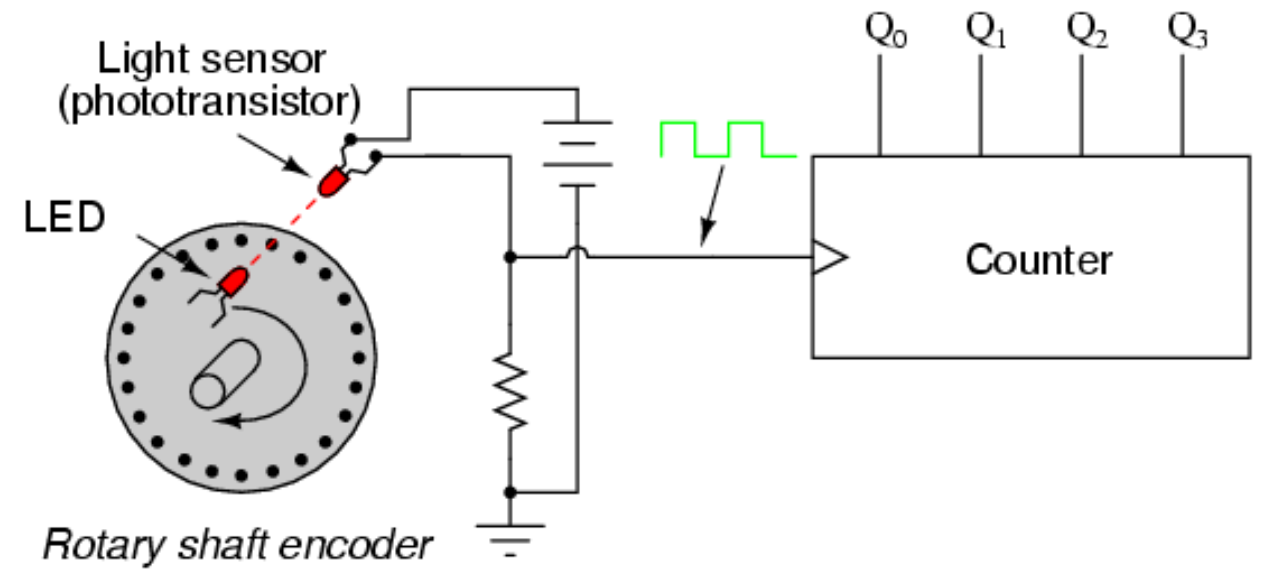
\includegraphics[width=0.6\textwidth]{figures/software/qei_demo.png}
    \caption {Principle of a rotary shaft encoder \cite{alex}}
    \label{fig:qei_demo}
\end{figure}

Whenever the wheel is rotated, light emitted from the LED will hit the light sensor (phototransistor) if there is a hole between them. Light sensor and emitter are separated by the wheel seen in \ref{fig:qei_demo}.
The time passed between the phototransistor turning on after registering light and turning off again after the light disappears behind the wheel will determine the velocity of our motor.


\subsubsection*{Analogue-to-Digital Conversion(ADC)}

\subsubsection*{Direct Memory Access (DMA) - does this belong here?}

\subsubsection*{Universal Asynchronous Receiver Transmitter (UART)}
Our dsPIC33FJ64MC804 has a Universal Asynchronous Receiver Transmitter (UART)  module for serial port communication.
The UART can communicate with peripheral devices. 
In our case, we use it to commmunicate with an outside computer to send commands or read out values. This was especially useful to find fitting parameters for our gains in the controller logic (chapter).

\begin{figure}[htb]
    \centering
    \includegraphics[width=0.6\textwidth]{figures/software/uart_demo.png}
    \caption {String transmission of 8 bit characters with one start bit and one stop bit (no parity) \cite{alex}}
    \label{fig:uart_demo}
\end{figure}

Figure \ref{fig:uart_demo} shows the transmission of a string consisting of three characters. 
The dsPIC33FJ64MC804 allows us to specify the properties of our transmission. The most important settings:
\begin{itemize}
    \item Baud rate: 57.6 kbit/s
    \item Data Selection Bits: 8
    \item Parity bit: 0
    \item Stop bit: 1
\end{itemize}

In order to send out messages, we require another module. We therefore connect our microcontroller to the \textbf{HC-05 Bluetooth Module} (figure \ref{fig:hc_05} so that we can send messages to that module which again transfers those messages via bluetooth to our computer where we read out the values.

\begin{figure}[htb]
    \centering
    \begin{minipage}{.5\textwidth}
          \centering
            \includegraphics[width=.9\linewidth]{figures/software/uart_hc05.jpg}
              \caption{HC-05 Bluetooth Module}
                \label{fig:hc_05}
    \end{minipage}%
    \begin{minipage}{.5\textwidth}
          \centering
            \includegraphics[width=.9\linewidth]{figures/software/uart_plug.png}
              \caption{Connecting the HC-05 module to our microcontroller}
                \label{fig:wire_3}
    \end{minipage}
\end{figure}

The 3-wire UART as seen in figure \ref{fig:wire_3} shows our configuration for a full-duplex communication. The Bluetooth module sends out the message it gets on the reception line (Rx) and sends back messages to the microcontroller through its transmission line (Tx). To receive the message from our microcontroller, we need to connect our computer to the HC-05 module via bluetooth.

It is important to configure the baud rate of the HC-05 module in advance, such that it matches our microcontroller's baud rate. Also, in order to read out values, the baud rate on the PC we are reading from, must also match (in this case 57.6 kbit/s)

\subsection{Pin Mapping}
\textcolor{red}{
maybe a diagram of which peripheral maps to which pin
}


\subsection{Controller Design and Approach}

\textcolor{red}{
Here goes the whole logic of the mouse movement control (how should it behave when is faced with the wall or on contrary - with the gap in the labyrinth). PID controller design and the logic behind it.
}

\subsubsection{Proportional-Integral-Derivative Controller (PID)}

\subsubsection{State Machine}




\section{Summary of tests}

Here goes everything practical we could possibly test - for example the speeding curve of the motor, the temperature conditions of the board (when we'll solder it - whether it is able to work without overheating and such) 
Of course, the PID working values (such as the error convergence rate)
Possible subsections:\\
    - casing tests \\
    - schematic tests \\
    - software logic tests \\



\section{Implementation challenges} \label{chap:challenges}

During the whole implementation process we've faced a significant amount of challenges of a diverse nature. For a major part of them we were able to find a feasible solution that was implemented or at least managed to come up with some solution propositions. All the challenges can be split up in the application categories, which are listed below.

\subsection{Organizational challenges}

\begin{enumerate}
  \item Organization of groups
  \begin{itemize}
      \item Problem encountered:\\
      The main problem from the beginning of the practical course was to organize all the project members into equally skilled groups. The splitting principles were also not clear.
      \item Solution found:\\
      The first solution we came up with was to split up into two groups of three people, which proved efficient enough (or rather the inconveniences didn't show up) at the initial working stages such as acquiring the initial knowledge and getting familiar with the tools. After some time it became clear, that this group separation doesn't work anymore. Because the workload of the whole project which stretched throughout the remaining time was too much for three people to carry out, so it was decided to unite the groups and continue working on the project jointly. This changing of structure mid-project also led to further complications in regards to management within a group, which will be discussed next.
  \end{itemize}
  \item Organization and management within a group
   \begin{itemize}
      \item Problem encountered:\\
        In terms of the management within the group, the major problems that were encountered are: \\
        - Lack of high-level working plan and working structure that everyone can stick to.\\
        - No clear role assignment for the project members, lack of the task management.\\
        - Lack of day-to-day updates and communication.\\
        - No unified repository for everyone to work with and further complications tied with that (follows the problem with groups separation mentioned previously)
      \item Solution found:\\
        The solution that helped to fix (to some degree) the first two problems was to (following the unification of two groups into one single unit) get rid of the multitasking paradigm  and to assign some specific task or "area of expertise" to each member of the project. Thus, after such decentralization the need for a centralized high-level working plan was decreased, because each participant could organize the working process to fulfill own needs the best. This of course led to deepening the problem of lacking communication and the solution was not the most efficient in terms of implementation speed. 
        The communication problem - tied to the absence of a single unified repository for each project member to work with - was solved in the second half of the project using GitHub.

  \end{itemize}
\end{enumerate}

\subsection{Software design challenges}
\subsection{PCB design challenges}
\begin{enumerate}
  \item Missing knowledge of a PCB
    \begin{itemize}
      \item Problem encountered:\\
      As it was mentioned in earlier stages of this document, at the beginning of this project, all of us didn't know how to design or even build a PCB board due to lack of knowledge in electrical engineering. 
      \item Solution found:\\
      During the practical course we learned the basics of how a schematic has to look like by rebuilding the schematic of the "dsPIC30F4011 Prototype Design" from scratch onto a breadboard. We sometimes also had to have a look at lasts year's micromouse PCB board for reference of placing several parts. 
    \end{itemize}
  \item Design of the final schematic and PCB
    \begin{itemize}
      \item Problem encountered:\\
      The overall process of designing the complete board took at approx. five to six weeks, which is far too long than we had anticipated. One of the main issues was the identification of the correct electronic components we needed for the board. The constraint was to only order parts from RSComponents, but not every component we had found was offered by them.
      Another time-consuming act was the decision of how to place all components so their elecromagnetic interference won't interfere with each other.
      \item Solution found:\\
      Most of the components we needed were already used by us in the practical course, hence we could copy them and their placement from the "dsPIC30F4011 Prototype Design" schematic. The main difference was that we changed the microcontroller to a dsPIC33FJ64MC804 - with almost double the amounts of pins, which didn't made it easier to design. But still we had to find a proper way of placing all components on the PCB which doesn't take too much space and doesn't lead to interfering parts.
    \end{itemize}
  \item Tracing of the PCB
    \begin{itemize}
      \item Problem encountered:\\
      We had to take into account the limited space we had on the board plus the correct size of the tracing for the several circuits. For example the tracing for the 9V battery circuit had to be bigger in size because of the higher possible current than on the 5V and 3.3V circuits.
      Another difficulty was to connect all pins according to the schematic due to the high amount of traces we needed. The finishing touch was to draw traces by using as few as possible vias.
      \item Solution found:\\
      After revising each iteration after another and talking to our professor, we finally reached a final state which was satisfactory for all of us. Although not all vias could be avoided, in the end we created a clean layout for the tracing.
    \end{itemize}
  \item Using Autodesk Eagle
    \begin{itemize}
      \item Problem encountered:\\
      Autodesk Eagle is a huge software environment for creating schematics and its counterpart the PCB - which no one of the team had ever used before. This means that we encountered a lot of problems on how to find the correct parts within the "Parts Library" and later on in the added "SamacSys Library". We had difficulties in selecting the correct parts which we used later on in the final version, and no idea whether the placement of the components is right or not. 
      \item Solution found:\\
      Through self-learning and literally trying out functionalities we managed to use Eagle as we pleased. In the end we had two experts for Eagle within our team, which did the part selection, placement and tracing of the components.
    \end{itemize}
\end{enumerate}

\subsection{Casing design challenges}

\begin{enumerate}
  \item Coordination with PCB Design
  \begin{itemize}
      \item Problem encountered:\\
      For design processes that are in parallel to each other, it is unavoidable to go back and forth. The challenge is to make modifications to the design without causing too much unnecessary work, as these modifications can happen quite frequently and making changes to existing design can often be error-prone.
      \item Solution found:\\
      One solution is to take advantage of “Parameters” feature of Fusion 360. To effectively utilising this feature, we need to make sure that non-critical dimensions are built upon these selected ones in a logical fashion, this is the key idea of parameter centric design approach. Since Fusion 360 provides an easy interface for modifying set parameters and automatically updates any design dimensions that are constrained upon these parameters, it can be a chain reaction after each modification to parameters. A set of effectively selected parameters not only ensures that we can modify the design according to our needs even later in the process, but also eliminates or at least minimises excessive manual modification.
      
      For example, when choosing the position of the motor’s central point, there are many things that can influence or change our decision, such as the dimension of the wheel and the clearance height from the floor that is necessary. One logical thing to do is to design the motor mount, through holes for the screws fastening the motor based on this motor position and set this position as our “parameter”. In this way if the wheel’s dimension is somehow changed, and we need to change the position of the motor, only slight modification to this “parameter” is needed, and Fusion 360 will automatically update the position of the motor mount etc.
  \end{itemize}
  \item Design for Tolerance
  \begin{itemize}
      \item Problem encountered:\\
      Any mechanical design of parts needs to take into account tolerance of dimensional errors. With the FDM 3D printer that we used providing a dimensional accuracy of lower limit of around  ± 0.5 mm, and ordered parts such as the distance sensor having a (default) tolerance of ± 0.3 mm \cite{sens}, it is worth paying attention when designing for fitting these parts to the casing.
      \item Solution found:\\
      The solution is quite straightforward, it is to design for the maximum error, and leave enough room for a tight fit. One exception is the case snap fit, where the clearance between two fit structures is 0.4 mm as recommended in [  ].
      
  \end{itemize}
  \item Design for 3D Printing
  \begin{itemize}
      \item Problem encountered:\\
      3D printing is a relatively fast and cheap way to produce prototypes, but it comes with its limitations. The 3D printing method we used (FDM) requires certain support structures to be added if there are steep overhanging parts, because heated and fluid material can not be deposited onto thin air. Without support structure, the print would deform and sometimes cause print fail. If support structures are used, removing such structures will leave the surface rough.
      \item Solution found:\\
      To alleviate such problem, it is firstly important to be mindful of the limitations that come with 3D printing, when designing parts that are supposed to be 3D printed. Avoid support structure as much as possible, one helpful thing to keep in mind is the 45 degree rule of FDM printing. It is said that FDM 3D printers can handle a overhanging structure of 45 degree, larger than that the print will deform. Therefore, by utilising this design rule, many overhanging structures can be avoided. Since support structures leave rough edges, it is important to identify the critical surfaces that require a high precision and accuracy to not have support structures, these surfaces are called critical surfaces. These critical surfaces are identified, such as inside wall of sensor casing, and designed in a way that they do not need support structures. However, it is sometimes difficult to avoid such support structures, it is then best to place support structures on non-critical surfaces, so that the negative consequence is only optical rather than functional.
      
      Second, when printing, a well chosen printing configuration can also help. Sometimes just by rotating the angle, at which the part is printed, can save a lot of support structures, by utilising the 45 degree rule.
      
      Lastly, when support structures are unavoidable, for example when there is a ring like structure, it would then be necessary to post-process the printed part by sanding, polishing etc.
  \end{itemize}
\end{enumerate}

\textcolor{red}{
Well, here go all the problems we faced coupled with our solutions for them. Potentially the longest part in the report. Can be split in parts similarly to the previous sections (talking about software, board and casing)
}

\section{Conclusions}

The actual and final result which was achieved is not perfect, but a great step towards a running "Micromouse" was accomplished. From the fact that no team member had proficiency in electrical engineering, when this project was started, one can say, that by dividing this challenge into three groups the result couldn't have been better (regarding the time constraint). \\
All in all, the project was a success regarding our lack of knowledge and by comparing it to the outcome. Also, a lot of new skills were learned by all team members.\\

\noindent
As the challenge was divided into three groups - Hardware, Software and Casing - one clearly can see the resulted outcome:
\begin{itemize}
    \item a printed PCB
    \item all ordered electrical components
    \item a working software
    \item a 3D-printed case which holds the PCB, both motors and battery\\
\end{itemize}

\noindent
These are the next steps which have to be done:
\begin{itemize}
    \item soldering of all electrial components onto the PCB
    \item feeding the software into the microcontroller
    \item testing and adjusting of the sensors for front, left and right
    \item writing the algorithm to find the center of a maze
\end{itemize}

\subsection{Proposals}

\begin{itemize}
    \item It would have been great to have a reference recommendation for everything that came up along the way. We know that we got our hands on many different subjects and issues. Even though, it would be nice to provide a reference for everything, from book chapters to articles or papers. For example, the document provided in the beginning was an excellent start, which unfortunately didn't cover much of electronics. This would help inexperienced students catch up with some extra effort and prove to be invaluable for referencing in the final report. All in all, I would use the book "Art of Electronics" for specific referencing.
    \item Have a presentation in the middle of the term. We believe the presentation pushed everyone and we really understood what is going on and what the progress is. We believe a midterm evaluation of the progress would help motivate more work and identify still missing points of the project.
    \item For students who don't have the knowledge yet to build a complete robot from scratch, it would have been nice to have more options to choose from. Although the course's name specifies that a robot is going to be "build from scratch", one still could introduce two kind of groups: One group which is building the hardware from scratch and another group which is responsible for the software and trying to optimize the search algorithm (by using a ready-to-use Micromouse).
\end{itemize}

\newpage
\section*{Glossary}

\begin{table}[H]
\begin{tabular}{ l l }
  RSComponents: & Seller of electrical components \\
  Mouser:       & Seller of electrical components \\
  SamacSys Library:     & A library used in Autodesk Eagle for electrical components \\
\end{tabular}
\end{table}
\vspace{3cm}

\bibliography{scibib}

\bibliographystyle{alpha}


\end{document}
